%\SweaveUTF8
\documentclass[aspectratio=169]{beamer}

\usetheme{default}
% Slide setup, colour independent

\usepackage{amsmath,amssymb,amsthm}
\usepackage[utf8]{inputenc}
\usepackage{colortbl}
\usepackage{bm}
\usepackage{xcolor}
\usepackage{dsfont}
\usepackage{setspace}
%\usepackage{subfigure}
% To use \ding{234} and the like
\usepackage{pifont}
% To cross reference between slide files
\usepackage{zref-xr,zref-user}
% Use something like
% \zexternaldocument{fileI}
% in the tex files. And cite using \zref instead of \ref
\usepackage{booktabs}
\usepackage{marvosym}
\usepackage{cancel}
%\usepackage{transparent}

% Fields and the like
\def\IC{\mathbb{C}}
\def\IE{\mathbb{E}}
\def\IF{\mathbb{F}}
\def\II{\mathbb{I}}
\def\IJ{\mathbb{J}}
\def\IK{\mathbb{K}}
\def\IM{\mathbb{M}}
\def\IN{\mathbb{N}}
\def\IP{\mathbb{P}}
\def\IR{\mathbb{R}}
\def\IZ{\mathbb{Z}}
\def\11{\mathds{1}}


% Bold lowercase
\def\ba{\bm{a}}
\def\bb{\bm{b}}
\def\bc{\bm{c}}
\def\bd{\bm{d}}
\def\be{\bm{e}}
\def\bf{\bm{f}}
\def\bh{\bm{h}}
\def\bi{\bm{i}}
\def\bj{\bm{j}}
\def\bk{\bm{k}}
\def\bn{\bm{n}}
\def\bp{\bm{p}}
\def\br{\bm{r}}
\def\bs{\bm{s}}
\def\bu{\bm{u}}
\def\bv{\bm{v}}
\def\bw{\bm{w}}
\def\bx{\bm{x}}
\def\by{\bm{y}}
\def\bz{\bm{z}}

% Bold capitals
\def\bB{\bm{B}}
\def\bD{\bm{D}}
\def\bE{\bm{E}}
\def\bF{\bm{F}}
\def\bG{\bm{G}}
\def\bI{\bm{I}}
\def\bL{\bm{L}}
\def\bN{\bm{N}}
\def\bP{\bm{P}}
\def\bR{\bm{R}}
\def\bS{\bm{S}}
\def\bT{\bm{T}}
\def\bX{\bm{X}}

% Bold numbers
\def\b0{\bm{0}}

% Bold greek
\bmdefine{\bmu}{\bm{\mu}}
\def\bphi{\bm{\phi}}
\def\bvarphi{\bm{\varphi}}
\def\bPi{\bm{\Pi}}
\def\bGamma{\bm{\Gamma}}

% Bold red sentence
\def\boldred#1{{\color{red}\textbf{#1}}}
\def\defword#1{{\color{orange}\textbf{#1}}}

% Caligraphic letters
\def\A{\mathcal{A}}
\def\B{\mathcal{B}}
\def\C{\mathcal{C}}
\def\D{\mathcal{D}}
\def\E{\mathcal{E}}
\def\F{\mathcal{F}}
\def\G{\mathcal{G}}
\def\H{\mathcal{H}}
\def\I{\mathcal{I}}
\def\L{\mathcal{L}}
\def\M{\mathcal{M}}
\def\N{\mathcal{N}}
\def\P{\mathcal{P}}
\def\R{\mathcal{R}}
\def\S{\mathcal{S}}
\def\T{\mathcal{T}}
\def\U{\mathcal{U}}
\def\V{\mathcal{V}}

% Adding space for prime (') where needed
\def\pprime{\,'}
% Adding space for star (\star) where needed
\def\pstar{{\,\star}}

% tt font for code
\def\code#1{{\tt #1}}

% i.e., e.g.
\def\eg{\emph{e.g.}}
\def\ie{\emph{i.e.}}


% Operators and special symbols
\def\nbOne{{\mathchoice {\rm 1\mskip-4mu l} {\rm 1\mskip-4mu l}
{\rm 1\mskip-4.5mu l} {\rm 1\mskip-5mu l}}}
\def\cov{\ensuremath{\mathsf{cov}}}
\def\Var{\ensuremath{\mathsf{Var}\ }}
\def\Im{\textrm{Im}\;}
\def\Re{\textrm{Re}\;}
\def\det{\ensuremath{\mathsf{det}}}
\def\diag{\ensuremath{\mathsf{diag}}}
\def\nullspace{\ensuremath{\mathsf{null}}}
\def\nullity{\ensuremath{\mathsf{nullity}}}
\def\rank{\ensuremath{\mathsf{rank}}}
\def\range{\ensuremath{\mathsf{range}}}
\def\sgn{\ensuremath{\mathsf{sgn}}}
\def\Span{\ensuremath{\mathsf{span}}}
\def\tr{\ensuremath{\mathsf{tr}}}
\def\imply{$\Rightarrow$}
\def\restrictTo#1#2{\left.#1\right|_{#2}}
\newcommand{\parallelsum}{\mathbin{\!/\mkern-5mu/\!}}
\def\dsum{\mathop{\displaystyle \sum }}%
\def\dind#1#2{_{\substack{#1\\ #2}}}

\DeclareMathOperator{\GL}{GL}
\DeclareMathOperator{\Rel}{Re}
\def\Nt#1{\left|\!\left|\!\left|#1\right|\!\right|\!\right|}
\newcommand{\tripbar}{|\! |\! |}



% The beamer bullet (in base colour)
\def\bbullet{\leavevmode\usebeamertemplate{itemize item}\ }

% Theorems and the like
\newtheorem{proposition}[theorem]{Proposition}
\newtheorem{property}[theorem]{Property}
\newtheorem{importantproperty}[theorem]{Property}
\newtheorem{importanttheorem}[theorem]{Theorem}
%\newtheorem{lemma}[theorem]{Lemma}
%\newtheorem{corollary}[theorem]{Corollary}
\newtheorem{remark}[theorem]{Remark}
\setbeamertemplate{theorems}[numbered]
%\setbeamertemplate{theorems}[ams style]

%
%\usecolortheme{orchid}
%\usecolortheme{orchid}

\def\red{\color[rgb]{1,0,0}}
\def\blue{\color[rgb]{0,0,1}}
\def\green{\color[rgb]{0,1,0}}


% Get rid of navigation stuff
\setbeamertemplate{navigation symbols}{}

% Set footline/header line
\setbeamertemplate{footline}
{%
\quad p. \insertpagenumber \quad--\quad \insertsection\vskip2pt
}
% \setbeamertemplate{headline}
% {%
% \quad\insertsection\hfill p. \insertpagenumber\quad\mbox{}\vskip2pt
% }


\makeatletter
\newlength\beamerleftmargin
\setlength\beamerleftmargin{\Gm@lmargin}
\makeatother

% Colours for special pages
\def\extraContent{yellow!20}


%%%%%%%%%%%%%%%%%
\usepackage{tikz}
\usetikzlibrary{shapes,arrows}
\usetikzlibrary{positioning}
\usetikzlibrary{shapes.symbols,shapes.callouts,patterns}
\usetikzlibrary{calc,fit}
\usetikzlibrary{backgrounds}
\usetikzlibrary{decorations.pathmorphing,fit,petri}
\usetikzlibrary{automata}
\usetikzlibrary{fadings}
\usetikzlibrary{patterns,hobby}
\usetikzlibrary{backgrounds,fit,petri}
\usetikzlibrary{tikzmark}

\usepackage{pgfplots}
\pgfplotsset{compat=1.6}
\pgfplotsset{ticks=none}

\usetikzlibrary{decorations.markings}
\usetikzlibrary{arrows.meta}
\tikzset{>=stealth}

% For tikz
\tikzstyle{cloud} = [draw, ellipse,fill=red!20, node distance=0.87cm,
minimum height=2em]
\tikzstyle{line} = [draw, -latex']


%%% For max frame images
\newenvironment{changemargin}[2]{%
\begin{list}{}{%
\setlength{\topsep}{0pt}%
\setlength{\leftmargin}{#1}%
\setlength{\rightmargin}{#2}%
\setlength{\listparindent}{\parindent}%
\setlength{\itemindent}{\parindent}%
\setlength{\parsep}{\parskip}%
}%
\item[]}{\end{list}}


% Make one image take up the entire slide content area in beamer,.:
% centered/centred full-screen image, with title:
% This uses the whole screen except for the 1cm border around it
% all. 128x96mm
\newcommand{\titledFrameImage}[2]{
\begin{frame}{#1}
%\begin{changemargin}{-1cm}{-1cm}
\begin{center}
\includegraphics[width=108mm,height=\textheight,keepaspectratio]{#2}
\end{center}
%\end{changemargin}
\end{frame}
}

% Make one image take up the entire slide content area in beamer.:
% centered/centred full-screen image, no title:
% This uses the whole screen except for the 1cm border around it
% all. 128x96mm
\newcommand{\plainFrameImage}[1]{
\begin{frame}[plain]
%\begin{changemargin}{-1cm}{-1cm}
\begin{center}
\includegraphics[width=108mm,height=76mm,keepaspectratio]{#1}
\end{center}
%\end{changemargin}
\end{frame}
}

% Make one image take up the entire slide area, including borders, in beamer.:
% centered/centred full-screen image, no title:
% This uses the entire whole screen
\newcommand{\maxFrameImage}[1]{
\begin{frame}[plain]
\begin{changemargin}{-1cm}{-1cm}
\begin{center}
\includegraphics[width=\paperwidth,height=\paperheight,keepaspectratio]
{#1}
\end{center}
\end{changemargin}
\end{frame}
}

% This uses the entire whole screen (to include in frame)
\newcommand{\maxFrameImageNoFrame}[1]{
\begin{changemargin}{-1cm}{-1cm}
\begin{center}
\includegraphics[width=\paperwidth,height=0.99\paperheight,keepaspectratio]
{#1}
\end{center}
\end{changemargin}
}

% Make one image take up the entire slide area, including borders, in beamer.:
% centered/centred full-screen image, no title:
% This uses the entire whole screen
\newcommand{\maxFrameImageColor}[2]{
\begin{frame}[plain]
\setbeamercolor{normal text}{bg=#2!20}
\begin{changemargin}{-1cm}{-1cm}
\begin{center}
\includegraphics[width=\paperwidth,height=\paperheight,keepaspectratio]
{#1}
\end{center}
\end{changemargin}
\end{frame}
}


\usepackage{tikz}
\usetikzlibrary{patterns,hobby}
\usepackage{pgfplots}
\pgfplotsset{compat=1.6}
\pgfplotsset{ticks=none}

\usetikzlibrary{backgrounds}
\usetikzlibrary{decorations.markings}
\usetikzlibrary{arrows.meta}
\tikzset{>=stealth}

\tikzset{
  clockwise arrows/.style={
    postaction={
      decorate,
      decoration={
        markings,
        mark=between positions 0.1 and 0.9 step 40pt with {\arrow{>}},
   }}}}


% Beginning of a section
\newcommand{\newSectionSlide}[1]{
\begin{frame}[noframenumbering,plain]
  \begin{tikzpicture}[remember picture,overlay]
    \node[above right,inner sep=0pt,opacity=0.2] at (current page.south west)
    {
        \includegraphics[height=\paperheight,width=\paperwidth]{#1}
    };
  \end{tikzpicture}
  \setbeamercolor{section in toc}{fg=subsub_header_section}
  \setbeamerfont{section in toc}{size=\Large,series=\bfseries}
  \setbeamertemplate{section in toc shaded}[default][60]
  %\setbeamercolor{background canvas}{bg=section_colour}
  \tableofcontents[
    currentsection,
    sectionstyle=show/shaded,
    subsectionstyle=show/hide/hide,
    subsubsectionstyle=hide/hide/hide]
\end{frame}
\addtocounter{page}{-1}
}

% Beginning of a subsection
\newcommand{\newSubSectionSlide}[1]{
\begin{frame}[noframenumbering,plain]
  \begin{tikzpicture}[remember picture,overlay]
    \node[above right,inner sep=0pt,opacity=0.2] at (current page.south west)
    {
        \includegraphics[height=\paperheight,width=\paperwidth]{#1}
    };
  \end{tikzpicture}
  \setbeamercolor{section in toc}{fg=subsub_header_section}
  \setbeamerfont{section in toc}{size=\Large,series=\bfseries}
  \setbeamertemplate{section in toc shaded}[default][60]
  %\setbeamercolor{background canvas}{bg=section_colour}
  \tableofcontents[
    currentsection,
    sectionstyle=show/hide,
    subsectionstyle=show/shaded/hide,
    subsubsectionstyle=hide/hide/hide]
\end{frame}
\addtocounter{page}{-1}
}



   %%%%%%%%%%%
% To have links to parts in the outline
\makeatletter
\AtBeginPart{%
  \addtocontents{toc}{\protect\beamer@partintoc{\the\c@part}{\beamer@partnameshort}{\the\c@page}}%
}
%% number, shortname, page.
\providecommand\beamer@partintoc[3]{%
  \ifnum\c@tocdepth=-1\relax
    % requesting onlyparts.
    \makebox[6em]{Part #1:} \textcolor{green!30!blue}{\hyperlink{#2}{#2}}
    \par
  \fi
}
\define@key{beamertoc}{onlyparts}[]{%
  \c@tocdepth=-1\relax
}
\makeatother%

\newcommand{\nameofthepart}{}
\newcommand{\nupart}[1]%
    {   \part{#1}%
        \renewcommand{\nameofthepart}{#1}%
        {
          \setbeamercolor{background canvas}{bg=orange!50}
          \begin{frame}{#1}%\partpage 
          \hypertarget{\nameofthepart}{}\tableofcontents%
          \end{frame}
        }
    }


% The title page with figure
\newcommand{\titlepagewithfigure}[1]{%
\begin{frame}[noframenumbering,plain]
  \begin{tikzpicture}[remember picture,overlay]
    \node[above right,inner sep=0pt,opacity=0.2] at (current page.south west)
    {
        \includegraphics[height=\paperheight,width=\paperwidth]{#1}
    };
    \node[anchor=north east,
    inner sep=5pt,
    opacity=0.9] at (current page.north east)
    {
        
\includegraphics[width=0.2\textwidth]{FIGS/UM-logo-horizontal-CMYK.png}
    };
    \node[anchor=south, 
    align=justify, 
    text=black, 
    text width=1.1\textwidth,
    font=\footnotesize]  (land_acknowledgement)
    at (current page.south) 
    {The University of Manitoba campuses are located on original lands of Anishinaabeg, Ininew, Anisininew, Dakota and Dene peoples, and on the National Homeland of the Red River Métis.\\
    We respect the Treaties that were made on these territories, we acknowledge the harms and mistakes of the past, and we dedicate ourselves to move forward in partnership with Indigenous communities in a spirit of Reconciliation and collaboration.};  
    \node[align=center, anchor=south,
    above=0.5cm of land_acknowledgement,
    text=black,
    font=\bfseries] {Fall 2024};
\end{tikzpicture}
  \setbeamercolor{title}{fg=subsub_header_section}
  \setbeamercolor{author}{fg=subsub_header_section} 
  \setbeamerfont{title}{size=\Large,series=\bfseries}
  \setbeamerfont{author}{size=\Large,series=\bfseries}
  \setbeamerfont{date}{series=\bfseries}
	\titlepage
\end{frame}
\addtocounter{page}{-1}
}


% The outline page, with figure
\newcommand{\outlinepage}[1]{%
\begin{frame}[noframenumbering,plain]
  \begin{tikzpicture}[remember picture,overlay]
    \node[above right,inner sep=0pt,opacity=0.2] at (current page.south west)
    {
        \includegraphics[height=\paperheight,width=\paperwidth]{#1}
    };
  \end{tikzpicture}
  \setbeamercolor{section in toc}{fg=subsub_header_section}
  \setbeamerfont{section in toc}{size=\Large,series=\bfseries}
  \frametitle{\textcolor{blue}{\LARGE\bfseries Outline}}
  \tableofcontents[hideallsubsections]
\end{frame}
\addtocounter{page}{-1}
}




\usecolortheme{orchid}
%% Listings
\usepackage{listings}
\definecolor{mygreen}{rgb}{0,0.6,0}
\definecolor{mygray}{rgb}{0.5,0.5,0.5}
\definecolor{mymauve}{rgb}{0.58,0,0.82}
\definecolor{mygold}{rgb}{1,0.843,0}
\definecolor{myblue}{rgb}{0.537,0.812,0.941}

\definecolor{mygold2}{RGB}{120,105,22}
\definecolor{mygrey2}{RGB}{50,50,50}

\definecolor{lgreen}{rgb}{0.6,0.9,.6}
\definecolor{lred}{rgb}{1,0.5,.5}

\lstloadlanguages{R}
\lstset{ %
  language=R,
  backgroundcolor=\color{black!05},   % choose the background color
  basicstyle=\footnotesize\ttfamily,        % size of fonts used for the code
  breaklines=true,                 % automatic line breaking only at whitespace
  captionpos=b,                    % sets the caption-position to bottom
  commentstyle=\color{mygreen},    % comment style
  escapeinside={\%*}{*)},          % if you want to add LaTeX within your code
  keywordstyle=\color{red},       % keyword style
  stringstyle=\color{mygold},     % string literal style
  keepspaces=true,
  columns=fullflexible,
  tabsize=4,
}
% Could also do (in lstset)
% basicstyle==\fontfamily{pcr}\footnotesize
\lstdefinelanguage{Renhanced}%
  {keywords={abbreviate,abline,abs,acos,acosh,action,add1,add,%
      aggregate,alias,Alias,alist,all,anova,any,aov,aperm,append,apply,%
      approx,approxfun,apropos,Arg,args,array,arrows,as,asin,asinh,%
      atan,atan2,atanh,attach,attr,attributes,autoload,autoloader,ave,%
      axis,backsolve,barplot,basename,besselI,besselJ,besselK,besselY,%
      beta,binomial,body,box,boxplot,break,browser,bug,builtins,bxp,by,%
      c,C,call,Call,case,cat,category,cbind,ceiling,character,char,%
      charmatch,check,chol,chol2inv,choose,chull,class,close,cm,codes,%
      coef,coefficients,co,col,colnames,colors,colours,commandArgs,%
      comment,complete,complex,conflicts,Conj,contents,contour,%
      contrasts,contr,control,helmert,contrib,convolve,cooks,coords,%
      distance,coplot,cor,cos,cosh,count,fields,cov,covratio,wt,CRAN,%
      create,crossprod,cummax,cummin,cumprod,cumsum,curve,cut,cycle,D,%
      data,dataentry,date,dbeta,dbinom,dcauchy,dchisq,de,debug,%
      debugger,Defunct,default,delay,delete,deltat,demo,de,density,%
      deparse,dependencies,Deprecated,deriv,description,detach,%
      dev2bitmap,dev,cur,deviance,off,prev,,dexp,df,dfbetas,dffits,%
      dgamma,dgeom,dget,dhyper,diag,diff,digamma,dim,dimnames,dir,%
      dirname,dlnorm,dlogis,dnbinom,dnchisq,dnorm,do,dotplot,double,%
      download,dpois,dput,drop,drop1,dsignrank,dt,dummy,dump,dunif,%
      duplicated,dweibull,dwilcox,dyn,edit,eff,effects,eigen,else,%
      emacs,end,environment,env,erase,eval,equal,evalq,example,exists,%
      exit,exp,expand,expression,External,extract,extractAIC,factor,%
      fail,family,fft,file,filled,find,fitted,fivenum,fix,floor,for,%
      For,formals,format,formatC,formula,Fortran,forwardsolve,frame,%
      frequency,ftable,ftable2table,function,gamma,Gamma,gammaCody,%
      gaussian,gc,gcinfo,gctorture,get,getenv,geterrmessage,getOption,%
      getwd,gl,glm,globalenv,gnome,GNOME,graphics,gray,grep,grey,grid,%
      gsub,hasTsp,hat,heat,help,hist,home,hsv,httpclient,I,identify,if,%
      ifelse,Im,image,\%in\%,index,influence,measures,inherits,install,%
      installed,integer,interaction,interactive,Internal,intersect,%
      inverse,invisible,IQR,is,jitter,kappa,kronecker,labels,lapply,%
      layout,lbeta,lchoose,lcm,legend,length,levels,lgamma,library,%
      licence,license,lines,list,lm,load,local,locator,log,log10,log1p,%
      log2,logical,loglin,lower,lowess,ls,lsfit,lsf,ls,machine,Machine,%
      mad,mahalanobis,make,link,margin,match,Math,matlines,mat,matplot,%
      matpoints,matrix,max,mean,median,memory,menu,merge,methods,min,%
      missing,Mod,mode,model,response,mosaicplot,mtext,mvfft,na,nan,%
      names,omit,nargs,nchar,ncol,NCOL,new,next,NextMethod,nextn,%
      nlevels,nlm,noquote,NotYetImplemented,NotYetUsed,nrow,NROW,null,%
      numeric,\%o\%,objects,offset,old,on,Ops,optim,optimise,optimize,%
      options,or,order,ordered,outer,package,packages,page,pairlist,%
      pairs,palette,panel,par,parent,parse,paste,path,pbeta,pbinom,%
      pcauchy,pchisq,pentagamma,persp,pexp,pf,pgamma,pgeom,phyper,pico,%
      pictex,piechart,Platform,plnorm,plogis,plot,pmatch,pmax,pmin,%
      pnbinom,pnchisq,pnorm,points,poisson,poly,polygon,polyroot,pos,%
      postscript,power,ppoints,ppois,predict,preplot,pretty,Primitive,%
      print,prmatrix,proc,prod,profile,proj,prompt,prop,provide,%
      psignrank,ps,pt,ptukey,punif,pweibull,pwilcox,q,qbeta,qbinom,%
      qcauchy,qchisq,qexp,qf,qgamma,qgeom,qhyper,qlnorm,qlogis,qnbinom,%
      qnchisq,qnorm,qpois,qqline,qqnorm,qqplot,qr,Q,qty,qy,qsignrank,%
      qt,qtukey,quantile,quasi,quit,qunif,quote,qweibull,qwilcox,%
      rainbow,range,rank,rbeta,rbind,rbinom,rcauchy,rchisq,Re,read,csv,%
      csv2,fwf,readline,socket,real,Recall,rect,reformulate,regexpr,%
      relevel,remove,rep,repeat,replace,replications,report,require,%
      resid,residuals,restart,return,rev,rexp,rf,rgamma,rgb,rgeom,R,%
      rhyper,rle,rlnorm,rlogis,rm,rnbinom,RNGkind,rnorm,round,row,%
      rownames,rowsum,rpois,rsignrank,rstandard,rstudent,rt,rug,runif,%
      rweibull,rwilcox,sample,sapply,save,scale,scan,scan,screen,sd,se,%
      search,searchpaths,segments,seq,sequence,setdiff,setequal,set,%
      setwd,show,sign,signif,sin,single,sinh,sink,solve,sort,source,%
      spline,splinefun,split,sqrt,stars,start,stat,stem,step,stop,%
      storage,strstrheight,stripplot,strsplit,structure,strwidth,sub,%
      subset,substitute,substr,substring,sum,summary,sunflowerplot,svd,%
      sweep,switch,symbol,symbols,symnum,sys,status,system,t,table,%
      tabulate,tan,tanh,tapply,tempfile,terms,terrain,tetragamma,text,%
      time,title,topo,trace,traceback,transform,tri,trigamma,trunc,try,%
      ts,tsp,typeof,unclass,undebug,undoc,union,unique,uniroot,unix,%
      unlink,unlist,unname,untrace,update,upper,url,UseMethod,var,%
      variable,vector,Version,vi,warning,warnings,weighted,weights,%
      which,while,window,write,\%x\%,x11,X11,xedit,xemacs,xinch,xor,%
      xpdrows,xy,xyinch,yinch,zapsmall,zip},%
   otherkeywords={!,!=,~,$,*,\%,\&,\%/\%,\%*\%,\%\%,<-,<<-,_,/},%
   alsoother={._$},%
   sensitive,%
   morecomment=[l]\#,%
   morestring=[d]",%
   morestring=[d]'% 2001 Robert Denham
  }%

%%%%%%% 
%% Definitions in yellow boxes
\usepackage{etoolbox}
\setbeamercolor{block title}{use=structure,fg=structure.fg,bg=structure.fg!40!bg}
\setbeamercolor{block body}{parent=normal text,use=block title,bg=block title.bg!20!bg}

\BeforeBeginEnvironment{definition}{%
	\setbeamercolor{block title}{fg=black,bg=yellow!20!white}
	\setbeamercolor{block body}{fg=black, bg=yellow!05!white}
}
\AfterEndEnvironment{definition}{
	\setbeamercolor{block title}{use=structure,fg=structure.fg,bg=structure.fg!20!bg}
	\setbeamercolor{block body}{parent=normal text,use=block title,bg=block title.bg!50!bg, fg=black}
}
\BeforeBeginEnvironment{importanttheorem}{%
	\setbeamercolor{block title}{fg=black,bg=red!20!white}
	\setbeamercolor{block body}{fg=black, bg=red!05!white}
}
\AfterEndEnvironment{importanttheorem}{
	\setbeamercolor{block title}{use=structure,fg=structure.fg,bg=structure.fg!20!bg}
	\setbeamercolor{block body}{parent=normal text,use=block title,bg=block title.bg!50!bg, fg=black}
}
\BeforeBeginEnvironment{importantproperty}{%
	\setbeamercolor{block title}{fg=black,bg=red!50!white}
	\setbeamercolor{block body}{fg=black, bg=red!30!white}
}
\AfterEndEnvironment{importantproperty}{
	\setbeamercolor{block title}{use=structure,fg=structure.fg,bg=structure.fg!20!bg}
	\setbeamercolor{block body}{parent=normal text,use=block title,bg=block title.bg!50!bg, fg=black}
}

% Colour for the outline page
\definecolor{outline_colour}{RGB}{230,165,83}
%% Colours for sections, subsections aand subsubsections
\definecolor{section_colour}{RGB}{27,46,28}
\definecolor{subsection_colour}{RGB}{52,128,56}
\definecolor{subsubsection_colour}{RGB}{150,224,154}
\definecolor{subsub_header_section}{RGB}{196,44,27}
%\definecolor{mygold}{rgb}{1,0.843,0}
% Beginning of a section
% \AtBeginSection[]{
% 	{
% 	  \setbeamercolor{section in toc}{fg=mygold}
% 		\setbeamercolor{background canvas}{bg=section_colour}
% 		\begin{frame}[noframenumbering,plain]
% 			\framesubtitle{\nameofthepart Chapter \insertromanpartnumber \ -- \iteminsert{\insertpart}}
% 			\tableofcontents[
% 				currentsection,
% 				sectionstyle=show/shaded,
% 				subsectionstyle=show/hide/hide,
% 				subsubsectionstyle=hide/hide/hide]
% 		\end{frame}
% 	\addtocounter{page}{-1}
% 	%\addtocounter{framenumber}{-1} 
% 	}
% }


% % Beginning of a section
% \AtBeginSubsection[]{
% 	{
% 	  \setbeamercolor{section in toc}{fg=mygold}
% 		\setbeamercolor{background canvas}{bg=subsection_colour}
% 		\begin{frame}[noframenumbering,plain]
% 				\framesubtitle{\nameofthepart Chapter \insertromanpartnumber \ -- \iteminsert{\insertpart}}
% 				\tableofcontents[
% 					currentsection,
% 					sectionstyle=show/hide,
% 					currentsubsection,
% 					subsectionstyle=show/shaded/hide,
% 					subsubsectionstyle=show/hide/hide]
% 			\end{frame}
% 		\addtocounter{page}{-1}
% 	}
% }

% \newcommand{\newSubSectionSlide}[1]{
% \begin{frame}[noframenumbering,plain]
%   \begin{tikzpicture}[remember picture,overlay]
%     \node[above right,inner sep=0pt,opacity=0.2] at (current page.south west)
%     {
%         \includegraphics[height=\paperheight,width=\paperwidth]{#1}
%     };
%   \end{tikzpicture}
%   \setbeamercolor{section in toc}{fg=subsub_header_section}
%   \setbeamerfont{section in toc}{size=\Large,series=\bfseries}
%   \setbeamertemplate{section in toc shaded}[default][60]
%   \setbeamertemplate{subsection in toc shaded}[default][60]
%   %\setbeamercolor{background canvas}{bg=section_colour}
%   \tableofcontents[
%     currentsection,
%     sectionstyle=show/hide,
%     currentsubsection,
%     subsectionstyle=show/shaded/hide,
%     subsubsectionstyle=show/hide/hide]
% \end{frame}
% \addtocounter{page}{-1}
% }


% Beginning of a section
\AtBeginSubsubsection[]{
	{
	  \setbeamercolor{section in toc}{fg=subsub_header_section}
	  \setbeamercolor{subsubsection in toc}{fg=mygold2}
	  \setbeamercolor{subsubsection in toc shaded}{fg=mygrey2}
		\setbeamercolor{background canvas}{bg=subsubsection_colour}
		\begin{frame}[noframenumbering,plain]
				\framesubtitle{\nameofthepart Chapter \insertromanpartnumber \ -- \iteminsert{\insertpart}}
				\tableofcontents[
					currentsection,
					sectionstyle=show/hide,
					currentsubsection,
					subsectionstyle=show/hide/shaded
					currentsubsubsection]%,
					%subsubsectionstyle=hide/hide/shaded]
					%currentsubsubsection]
			\end{frame}
		\addtocounter{page}{-1}
	}
}


\title[Shallow water]{Shallow water\\[1.5cm] Partial differential equations}
\author{\texorpdfstring{Julien Arino\newline University of Manitoba\newline\url{julien.arino@umanitoba.ca}}{Julien Arino}}
\date{}


%%%%%%%%%%%%%%%%
\usepackage{Sweave}
\begin{document}
\input{math3610-07-shallow-water-concordance}




%%%%%%%%%%%%%%%%%%%%%%%%%%%%%%%%%
%%%%%%%%%%%%%%%%%%%%%%%%%%%%%%%%%
%%%%%%%%%%%%%%%%%%%%%%%%%%%%%%%%%
%%%%%%%%%%%%%%%%%%%%%%%%%%%%%%%%%
% The title page
\begin{frame}[noframenumbering,plain]
  \begin{tikzpicture}[remember picture,overlay]
    \node[above right,inner sep=0pt,opacity=0.2] at (current page.south west)
    {
        
\includegraphics[height=\paperheight,width=\paperwidth]{FIGS/population-models-Gemini_Generated_Image_r55bcer55bcer55b.jpeg}
    };
    \node[anchor=north east,
    inner sep=5pt,
    opacity=0.9] at (current page.north east)
    {
        
\includegraphics[width=0.2\textwidth]{FIGS/UM-logo-horizontal-CMYK.png}
    };
    \node[anchor=south, 
    align=justify, 
    text=black, 
    text width=1.1\textwidth,
    font=\footnotesize]  (land_acknowledgement)
    at (current page.south) 
    {The University of Manitoba campuses are located on original lands of Anishinaabeg, Ininew, Anisininew, Dakota and Dene peoples, and on the National Homeland of the Red River Métis.\\
    We respect the Treaties that were made on these territories, we acknowledge the harms and mistakes of the past, and we dedicate ourselves to move forward in partnership with Indigenous communities in a spirit of Reconciliation and collaboration.};  
    \node[align=center, anchor=south,
    above=0.5cm of land_acknowledgement,
    text=black,
    font=\bfseries] {Fall 2024};
\end{tikzpicture}
  \setbeamercolor{title}{fg=subsub_header_section}
  \setbeamercolor{author}{fg=subsub_header_section} 
  \setbeamerfont{title}{size=\Large,series=\bfseries}
  \setbeamerfont{author}{size=\Large,series=\bfseries}
  \setbeamerfont{date}{series=\bfseries}
	\titlepage
\end{frame}
\addtocounter{page}{-1}


%%%%%%%%%%%%%%%%%%%%%%%%%%%%%%%%%
%%%%%%%%%%%%%%%%%%%%%%%%%%%%%%%%%
%%%%%%%%%%%%%%%%%%%%%%%%%%%%%%%%%
%%%%%%%%%%%%%%%%%%%%%%%%%%%%%%%%%
% The outline page
\begin{frame}[noframenumbering,plain]
  \begin{tikzpicture}[remember picture,overlay]
    \node[above right,inner sep=0pt,opacity=0.2] at (current page.south west)
    {
        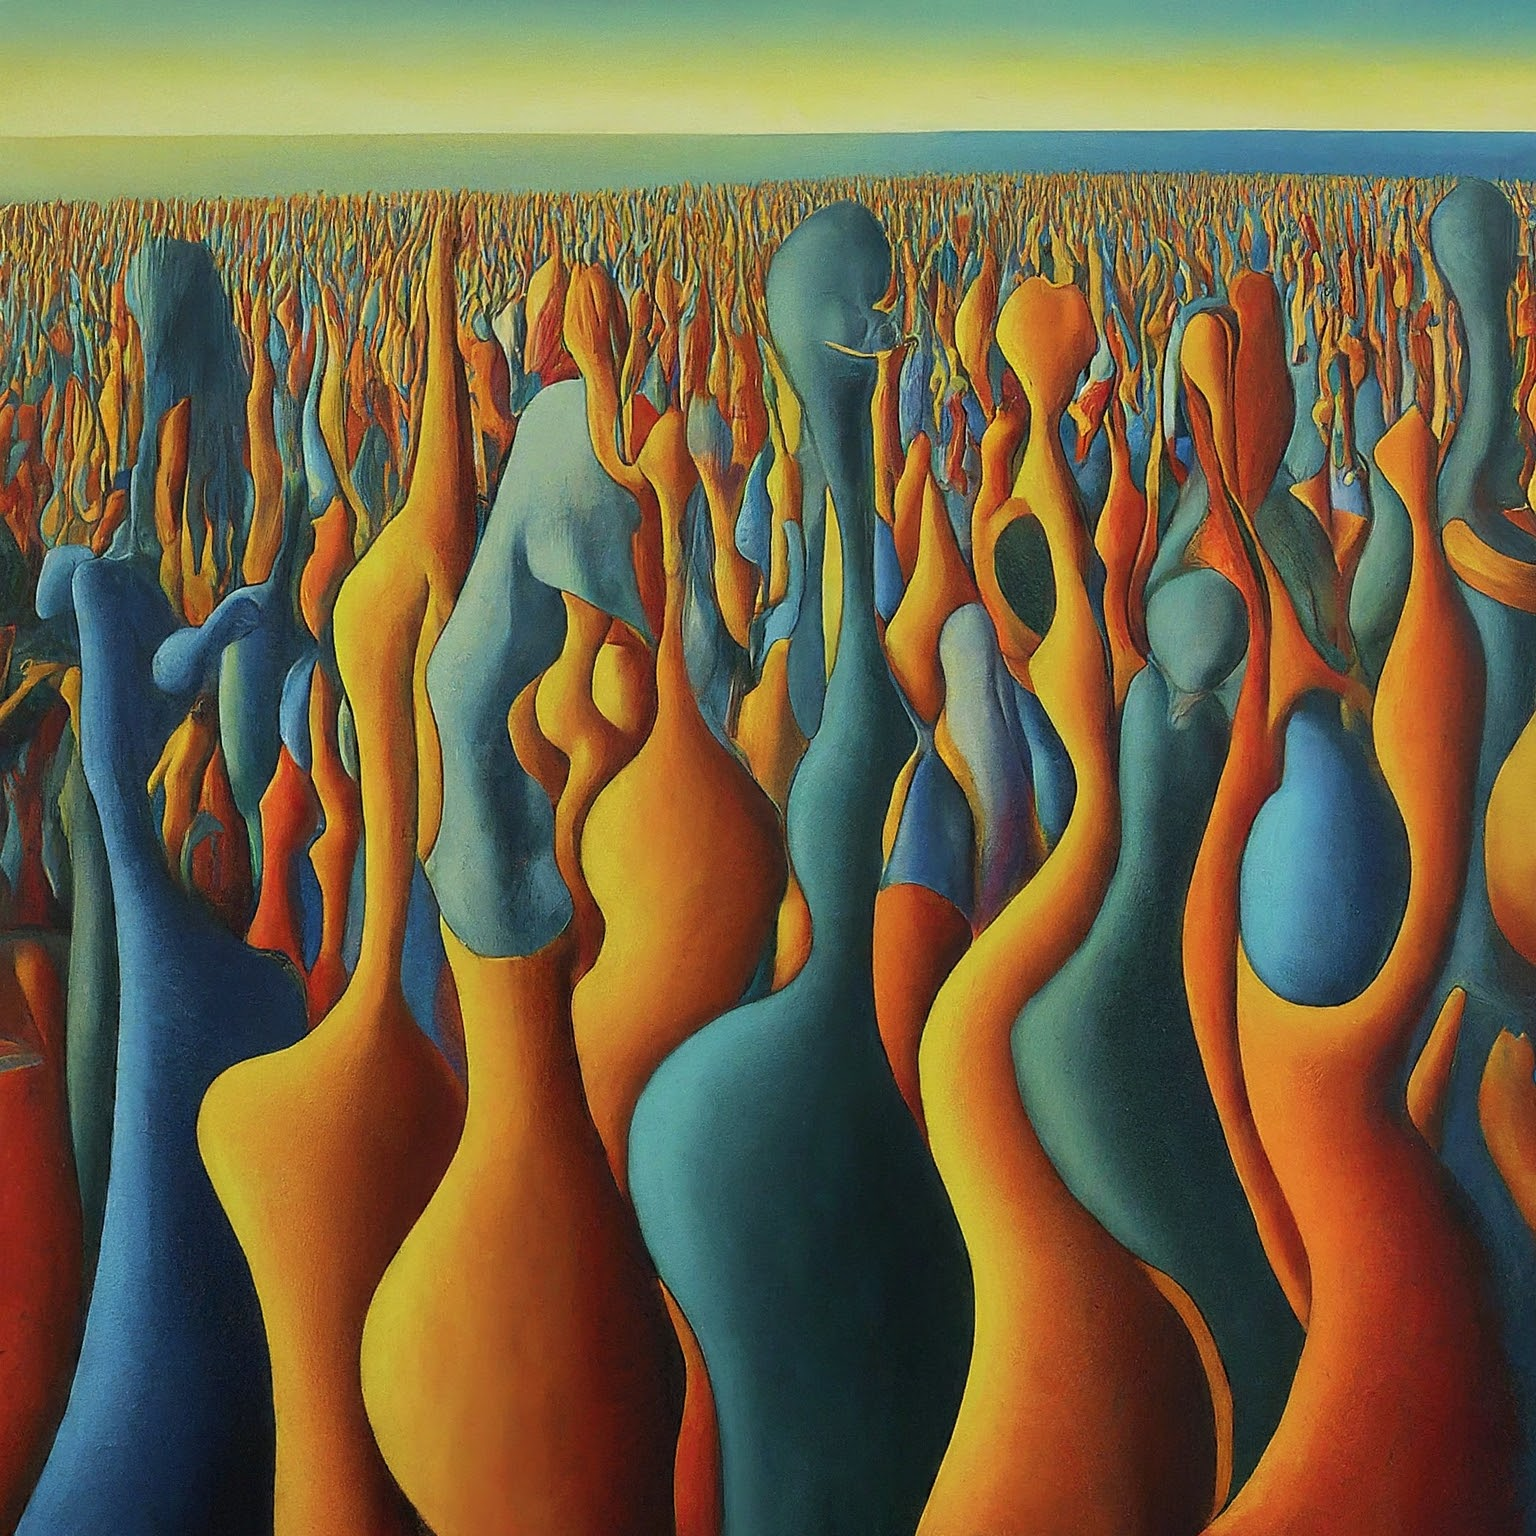
\includegraphics[height=\paperheight,width=\paperwidth]{FIGS/population-models-Gemini_Generated_Image_r55bccr55bccr55b.jpeg}
    };
  \end{tikzpicture}
  \setbeamercolor{section in toc}{fg=subsub_header_section}
  \setbeamerfont{section in toc}{size=\Large,series=\bfseries}
  \frametitle{\textcolor{blue}{\LARGE\bfseries Outline}}
  \tableofcontents[hideallsubsections]
\end{frame}
\addtocounter{page}{-1}



%%%%%%%%%%%%%%%%%%%
%%%%%%%%%%%%%%%%%%%
%%%%%%%%%%%%%%%%%%%
%%%%%%%%%%%%%%%%%%%
\section{Model formulation}
\frame[plain]{\tableofcontents[current]}

\frame{\frametitle{Spatial domain}
We consider the motion of a body of water that is infinite in the $z$ direction, with or without boundary in the $x$ direction, and the vertical direction of gravity taken as the $y$ direction.
\begin{center}
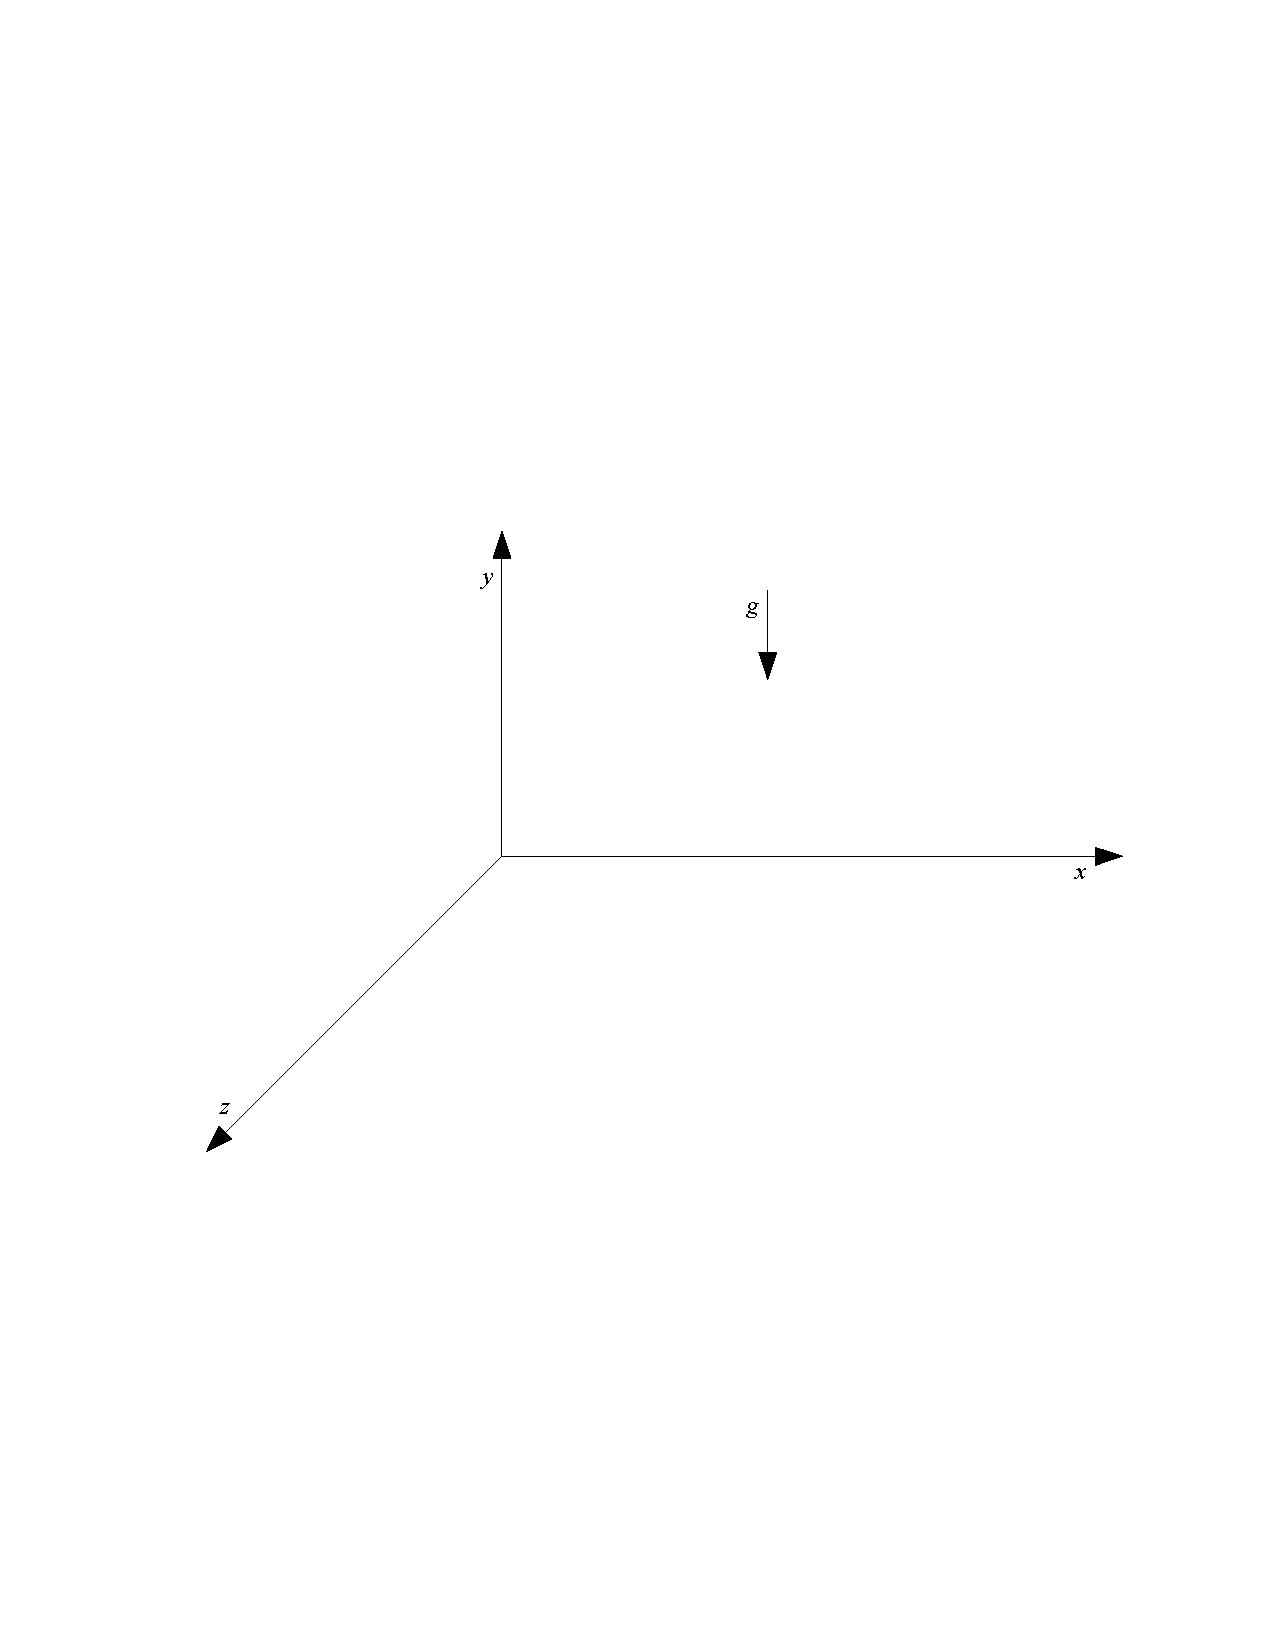
\includegraphics[width=0.7\textwidth]{FIGS/xyz_domain}
\end{center}
From now on, suppose $z$ direction uniform (the same for all $z$), so ignore $z$ except for the sake of argument.
}

\frame{
\begin{itemize}
\item Water depth at rest, $H$, small compared to distance $L_0$ over which significant changes can occur in the $x$ direction.
\item Undisturbed water surface, $y=0$.
\item Moving upper free surface $y=\eta$, measured from $y=0$.
\item Sea floor $y=-H$.
\end{itemize}
\begin{center}
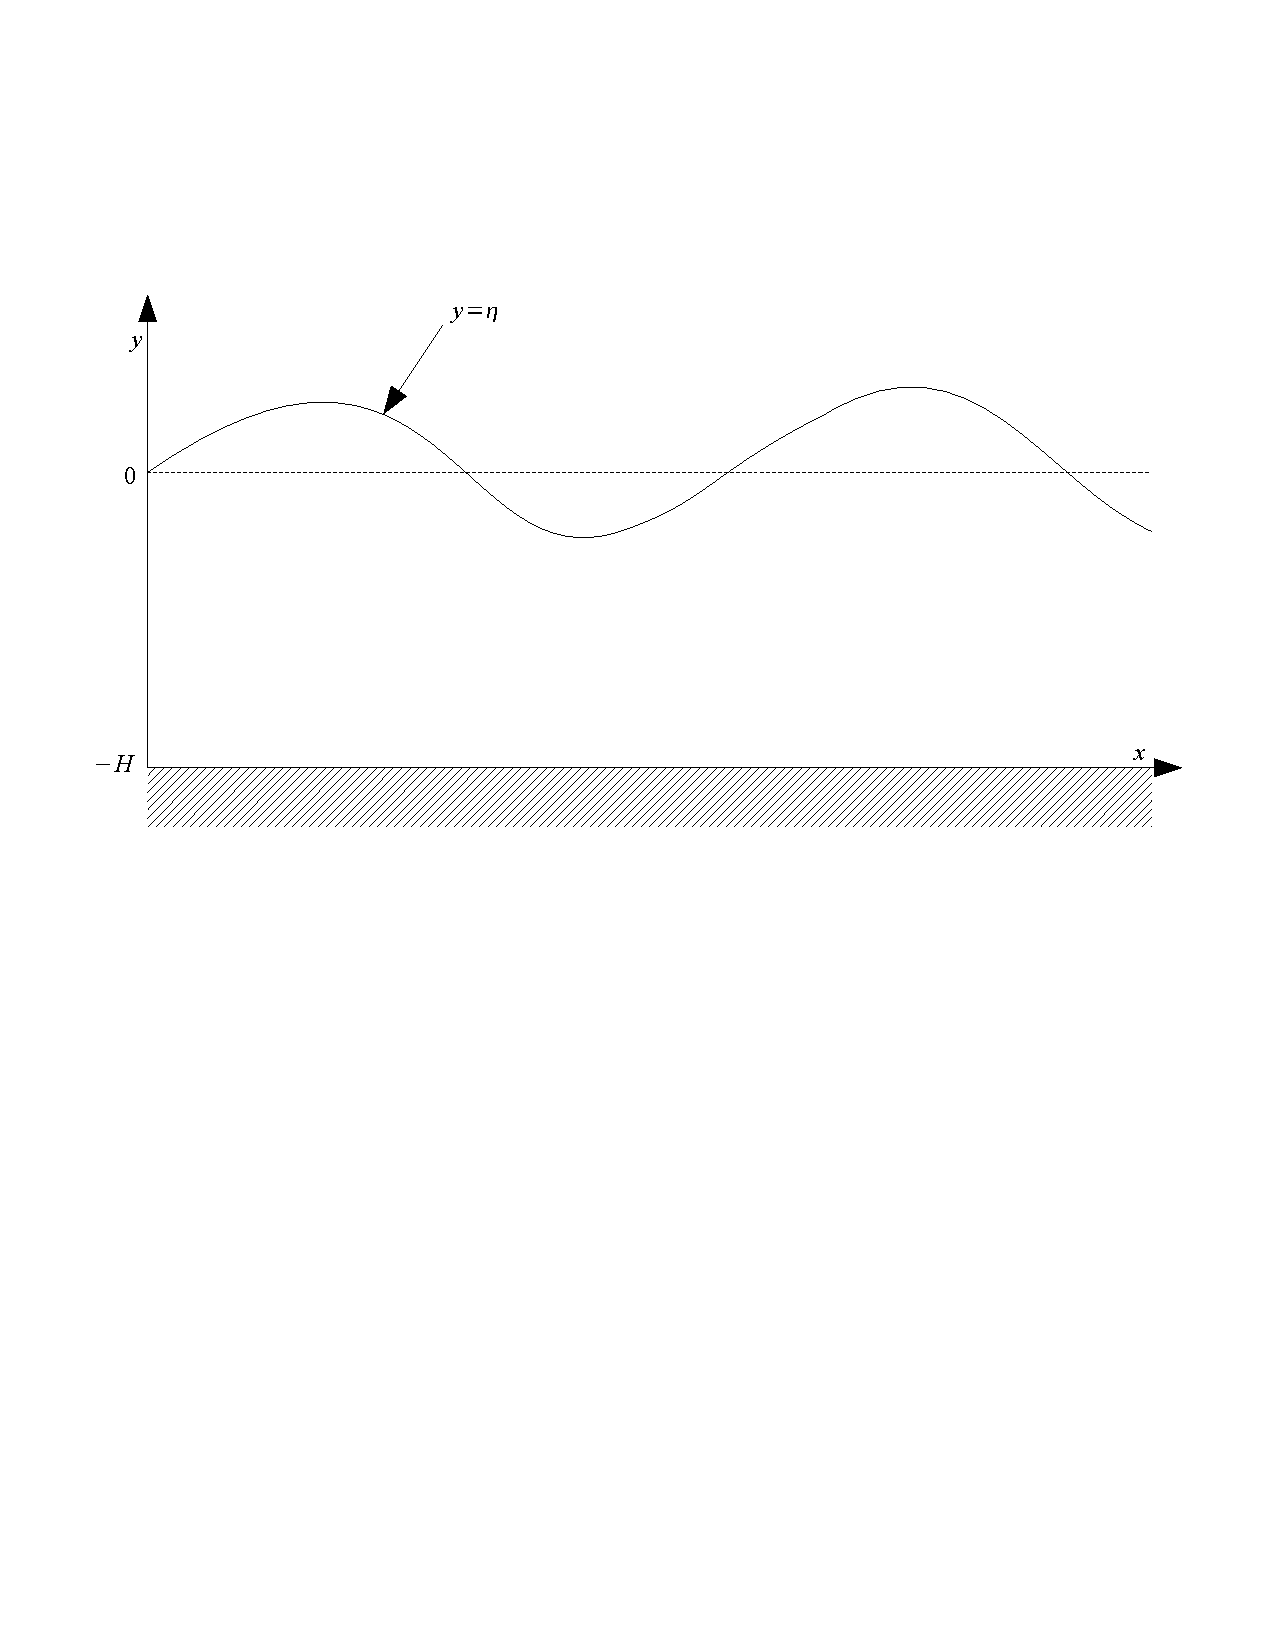
\includegraphics[width=0.7\textwidth]{FIGS/xy_domain}
\end{center}
}

\frame{
\begin{itemize}
\item $u$ velocity in the $x$ direction. Assume independent of depth $y$.
\item $\rho$ mass density of water.
\item $p(x,y,t)$ pressure in fluid at point $(x,y)$ at time $t$. In water, magnitude at any $(x,y)$ is same in all directions.
\end{itemize}
Fluid motion independent of $z$, so
\begin{itemize}
\item $u=u(x,t)$
\item $\eta=\eta(x,t)$.
\end{itemize}
}


\frame{
Take a cylindrical water column, with base area $A$, between $y_1$ and $y_2>y_1$.
\begin{center}
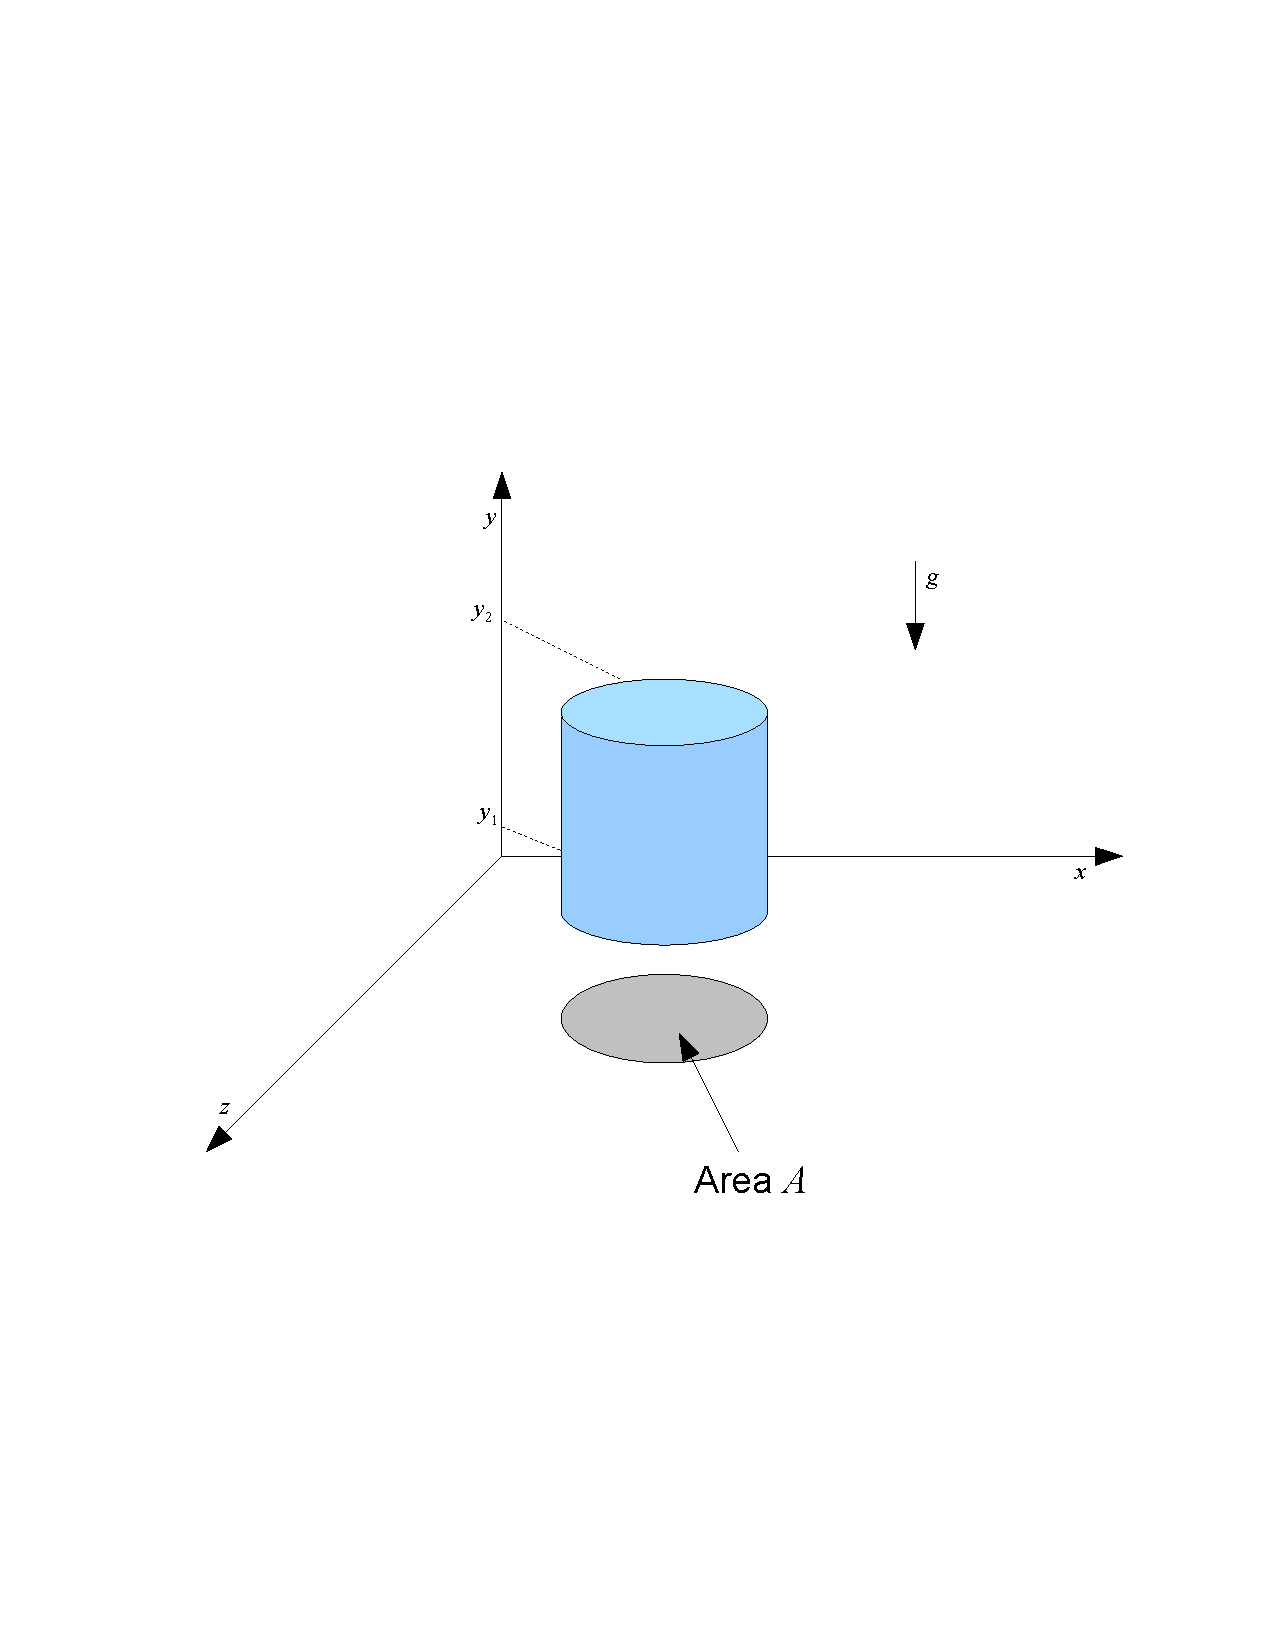
\includegraphics[width=0.7\textwidth]{FIGS/xyz_cylinder}
\end{center}
Force equilibrium in the $y$ direction in this cylinder requires balance of weight of water column and pressure differential between bottom face $y=y_1$ and top face $y=y_2$.
}

\frame{
Weight of water column:
\[
\mathop{\int\!\!\!\int}_A\int\limits_{y_1}^{y_2}(-\rho g)\ dydxdz
\]
Pressure differential:
\[
\mathop{\int\!\!\!\int}_A\left(p(x,y_2,t)-p(x,y_1,t)\right)\ dxdz
\]
So we must have
\[
\mathop{\int\!\!\!\int}_A\int\limits_{y_1}^{y_2}(-\rho g)\ dydxdz = \mathop{\int\!\!\!\int}_A\left(p(x,y_2,t)-p(x,y_1,t)\right)\ dxdz
\]
}

\frame{
\[
\mathop{\int\!\!\!\int}_A\int\limits_{y_1}^{y_2}(-\rho g)\ dydxdz = \mathop{\int\!\!\!\int}_A\left(p(x,y_2,t)-p(x,y_1,t)\right)\ dxdz
\]
is equivalent to
\[
\mathop{\int\!\!\!\int}_A\int\limits_{y_1}^{y_2}\left(\frac{\partial p}{\partial y}+\rho g\right)\ dydxdz=0
\]
This must be true for any water column, i.e., any $A,y_1,y_2$. Therefore,
\[
\frac{\partial p}{\partial y}+\rho g=0
\]
(otherwise, we would be able to find a water column where the integrand is positive, leading to a positive value of the integral on that column).
}


\frame{\frametitle{Water is incompressible}
If you force a body of water to deform, the volume of that body of water remains constant, i.e., water is an \emph{incompressible fluid}.
\vskip0.5cm
\noindent
$\Rightarrow$ $\rho$, the density, is a constant, and from
\[
\frac{\partial p}{\partial y}+\rho g=0
\]
we get
\[
p=-\rho g y+C,
\]
so if $p$ is measured relative to the pressure above the free upper surface $y=\eta$,
\[
p=\rho g(\eta-y)
\]
}


\frame{\frametitle{Water accumulation}
Consider a fixed volume $V$,
\[
V=\{z_1\leq z\leq z_2,x_1\leq x\leq x_2,-H\leq y\leq\eta\}
\]
\begin{center}
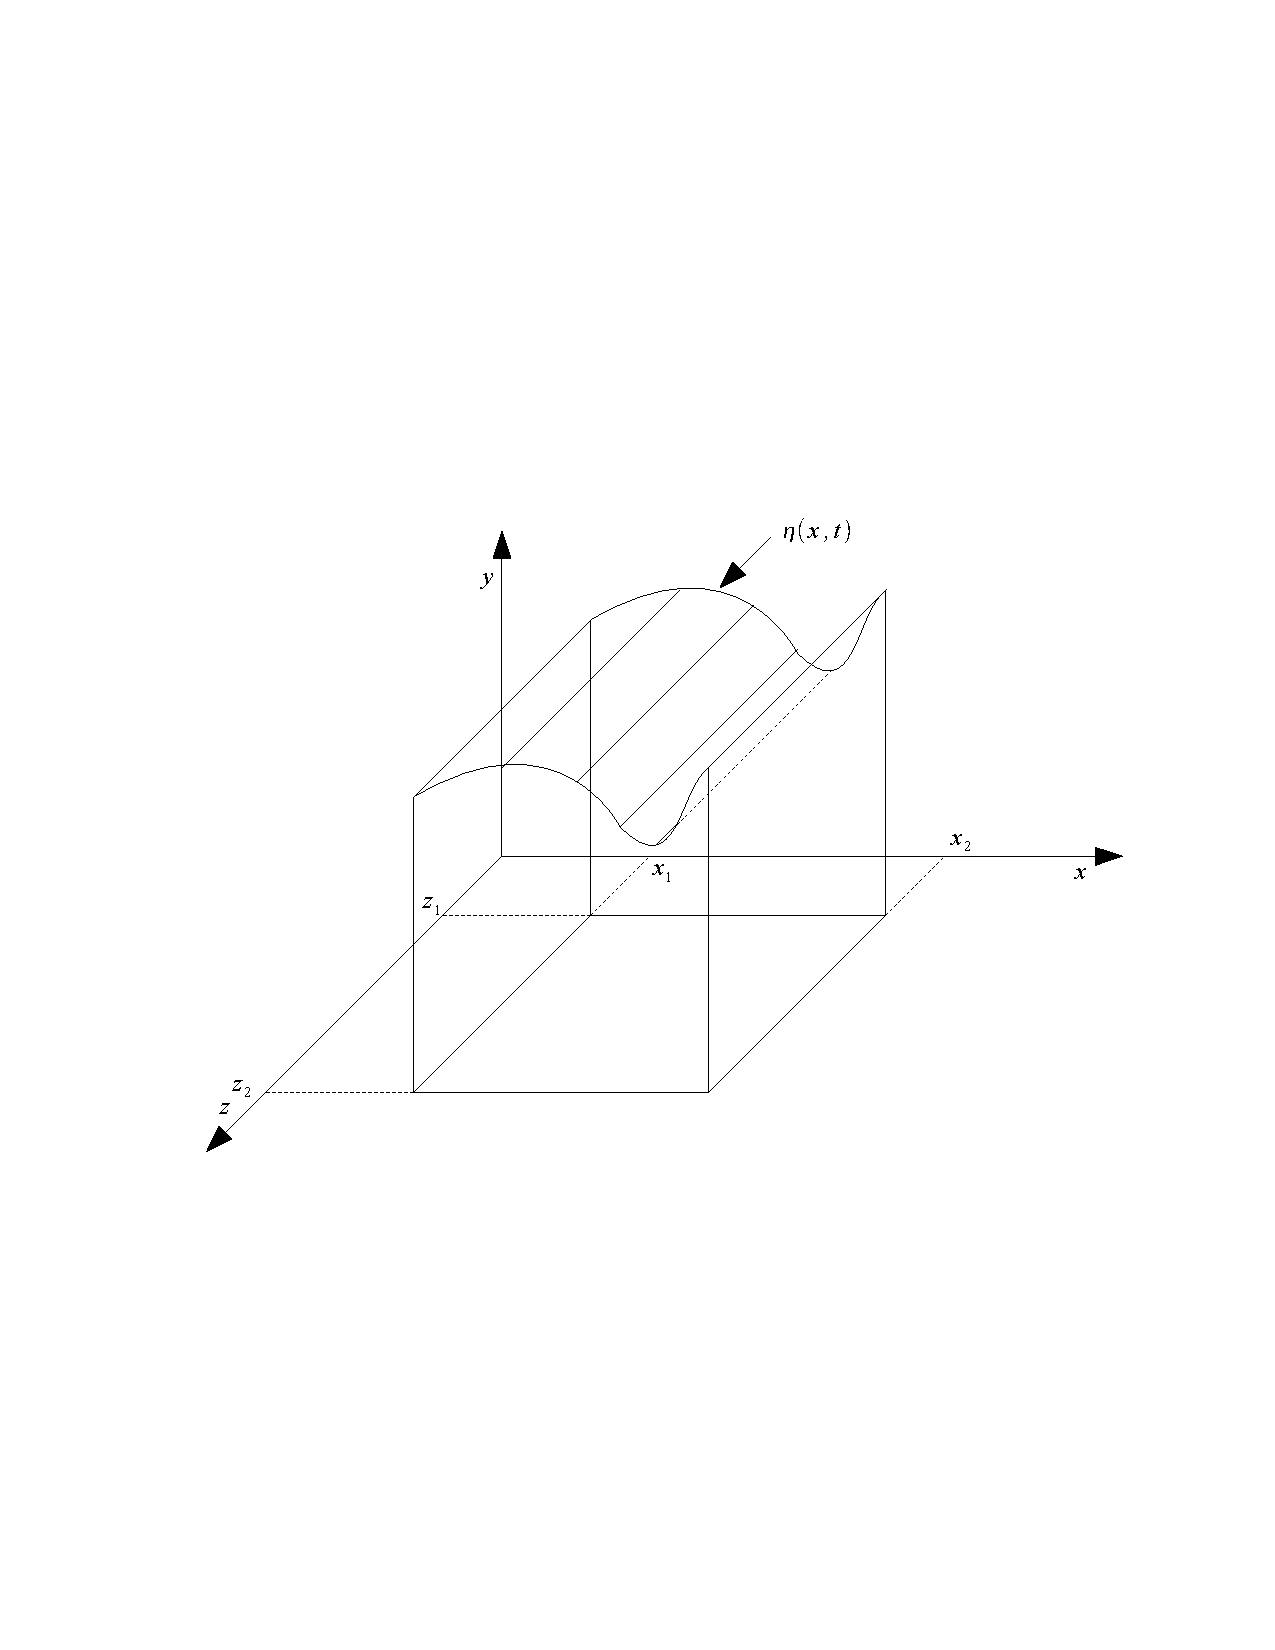
\includegraphics[width=0.7\textwidth]{FIGS/V_domain}
\end{center}
}

\frame{
Water enters $V$ through $x_1$ face and leaves $V$ through $x_2$ face. 
\begin{center}
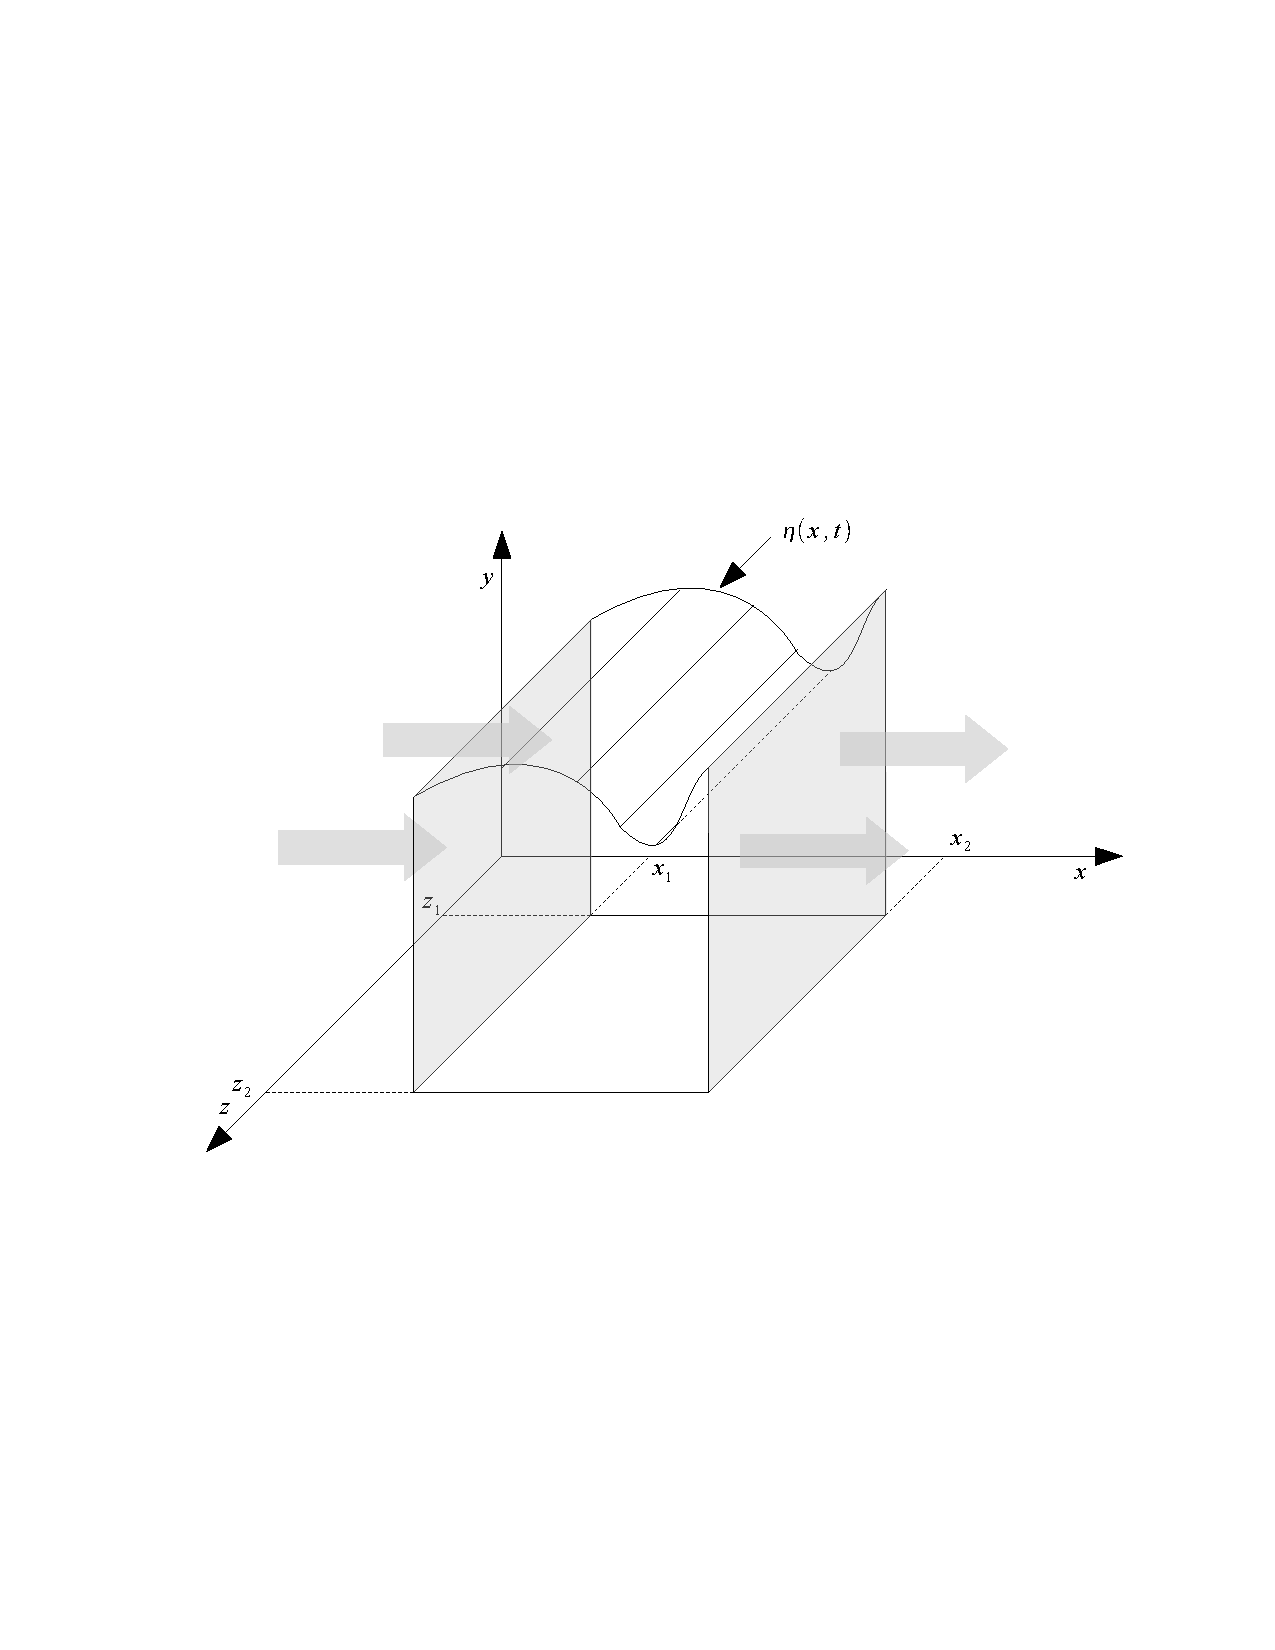
\includegraphics[width=0.7\textwidth]{FIGS/V_domain_flows}
\end{center}
Rate of water accumulation in $V$ is
\[
\frac{d}{dt}\int_{z_1}^{z_2}\int_{x_1}^{x_2}\int_{-H}^\eta \rho\ dydxdz =\Delta z\frac{d}{dt}\int_{x_1}^{x_2}\rho h\ dx,
\]
with $\Delta z=z_2-z_1$, and $h(x,t)=\eta+H$ the height of water at time $t$ at spatial location $x$.
}

\frame{\frametitle{Water flux}
Net flux of water entering $V$ through its faces $x=x_1$ and $x=x_2$ is
\begin{center}
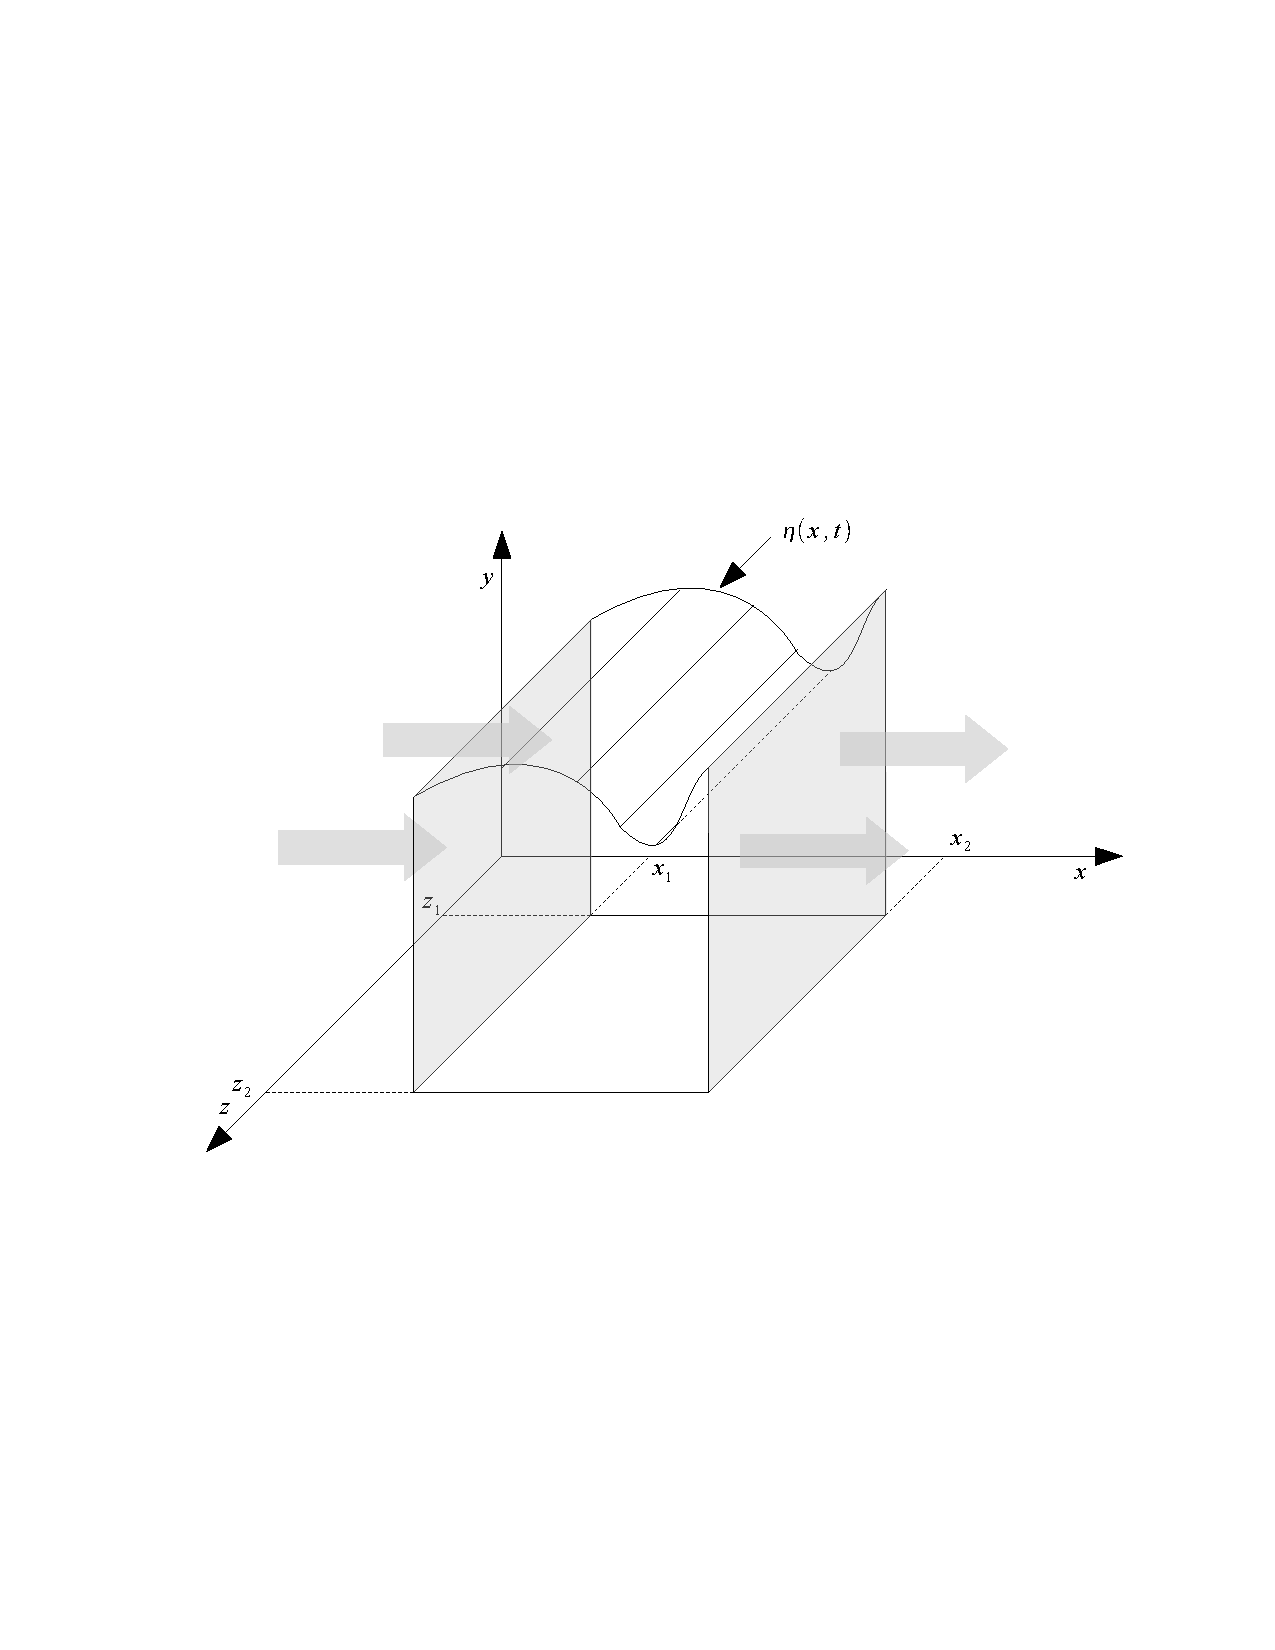
\includegraphics[width=0.7\textwidth]{FIGS/V_domain_flows}
\end{center}
\[
\left[\int_{z_1}^{z_2}\int_{-H}^\eta u\ dydz\right]_{x=x_1}
-\left[\int_{z_1}^{z_2}\int_{-H}^\eta u\ dydz\right]_{x=x_2} 
=-\Delta z\left[\rho uh\right]_{x_1}^{x_2}
\]
There is no flux through $y=-H$ and $y=\eta$, and no net flux through $z=z_1$ and $z=z_2$.
}

\frame{\frametitle{Conservation of mass}
Of course, the mass must conserve in $V$, so the two expressions must be equal, i.e.,
\[
\frac{d}{dt}\int\limits_{x_1}^{x_2} \rho h\ dx+\left[\rho uh\right]_{x_1}^{x_2}=0
\]
}

\frame{
Newton's second law for deformable media (Euler): rate of increase of horizontal momentum (in the $x$ direction) in $V$ must equal the sum of the net influx of momentum into the volume and the net horizontal force acting on the column.
\vskip0.2cm
(Momentum: product of mass and velocity of an object).
\vskip0.5cm
Rate of increase of momentum
\[
\frac{d}{dt}\int\limits_{z_1}^{z_2}\int\limits_{x_1}^{x_2}\int\limits_{-H}^\eta \rho u\ dydxdz
=\Delta z\frac{d}{dt}\int\limits_{x_1}^{x_2}\rho uh dx
\]
}

\frame{\frametitle{Momentum flux}
Net influx of momentum through faces $x=x_1$ and $x=x_2$ is
\begin{multline*}
\left[\int\limits_{z_1}^{z_2}\int\limits_{-H}^\eta (\rho u)u\ dydz\right]_{x=x_1}
-\left[\int\limits_{z_1}^{z_2}\int\limits_{-H}^\eta (\rho u)u\ dydz\right]_{x=x_2} \\
=-\Delta z\left[\rho u^2h\right]_{x_1}^{x_2}
\end{multline*}
There is no flux through $y=-H$ and $y=\eta$, and no net flux through $z=z_1$ and $z=z_2$.
}

\frame{\frametitle{Forces acting on $V$}
Ignore friction at $y=-H$. Then only contributions to horizontal forces come from pressure at $x=x_1$ and $x=x_2$, so net horizontal forces acting on $V$ is
\begin{align*}
\left[\int\limits_{z_1}^{z_2}\int\limits_{-H}^\eta p\ dydz\right]_{x_1}^{x_2} &=
-\left[\Delta z\int\limits_{-H}^\eta \rho g(\eta-y)\ dy\right]_{x_1}^{x_2} \\
&= \left[\left.-\Delta z\rho g(\eta y-\frac 12 y^2)\right|_{-H}^\eta\right]_{x_1}^{x_2} \\
&=\left[-\frac 12 \Delta z\rho g h^2\right]_{x_1}^{x_2}
\end{align*}
}

\frame{\frametitle{Conclusion from Newton's second law}
\[
\frac{d}{dt}\int\limits_{x_1}^{x_2}\rho uh\ dx
+\left[\rho u^2h+\frac 12\rho gh^2\right]_{x_1}^{x_2}=0
\]
}

\frame{\frametitle{The general model}
Pressure magnitude:
\begin{equation}\label{eq:pressure}
p=\rho g(\eta-y)
\end{equation}
Horizontal velocity:
\begin{equation}\label{eq:horiz_velocity}
\frac{d}{dt}\int\limits_{x_1}^{x_2} \rho h\ dx+\left[\rho uh\right]_{x_1}^{x_2}=0
\end{equation}
Free surface height:
\begin{equation}\label{eq:free_surf}
\frac{d}{dt}\int\limits_{x_1}^{x_2}\rho uh\ dx
+\left[\rho u^2h+\frac 12\rho gh^2\right]_{x_1}^{x_2}=0
\end{equation}
}


\section{Case of smooth solutions}
\frame[plain]{\tableofcontents[current]}


\frame{
Suppose $u$ and $h$ are smooth (with continuous first order partial derivatives),
then \eqref{eq:horiz_velocity} and \eqref{eq:free_surf} take a much simpler form,
\[
\int_{x_1}^{x_2}\left(\frac{\partial h}{\partial t}+\frac{\partial}{\partial x}(uh)\right)\ dx=0
\]
and
\[
\int_{x_1}^{x_2}\left(\frac{\partial}{\partial t}(uh)+\frac{\partial}{\partial x}(u^2h+\frac 	12gh^2)\right)\ dx=0
\]
Since the intervals of integration $[x_1,x_2]$ are arbitrary, and that the integrands are continuous, we have
\[
\frac{\partial h}{\partial t}+\frac{\partial}{\partial x}(uh)=0
\]
and
\[
\frac{\partial}{\partial t}(uh)+\frac{\partial}{\partial x}(u^2h+\frac 	12gh^2)=0
\]
}

\frame{
We write
\[
\frac{\partial h}{\partial t}+\frac{\partial}{\partial x}(uh)=0
\]
and
\[
\frac{\partial}{\partial t}(uh)+\frac{\partial}{\partial x}(u^2h+\frac 	12gh^2)=0
\]
as
\begin{align}
h_t+(uh)_x&=0 \label{eq:h2}\\
\intertext{and}
(uh)_t+(u^2h+\frac 12gh^2)_x &=0 \label{eq:u2}
\end{align}
}

\frame{
From \eqref{eq:h2},
\[
h_t=-(uh)_x=-(u_xh+uh_x)
\]
Equation \eqref{eq:u2} can be rewritten as
\begin{align*}
\eqref{eq:u2} &\Leftrightarrow u_th+uh_t+(u^2h+\frac 12gh^2)_x=0 \\
&\Leftrightarrow 
u_th-u(u_xh+uh_x)+2uu_xh+u^2h_x+ghh_x=0 \\
&\Leftrightarrow u_th-uu_xh-\cancel{u^2h_x}+2uu_xh+\cancel{u^2h_x}+ghh_x=0 \\
&\Leftrightarrow u_th+uu_xh+ghh_x=0
\end{align*}
Therefore, provided $h\neq 0$, we get
\begin{subequations}\label{sys:smooth}
\begin{align}
h_t+(uh)_x&=0 \label{eq:h}\\
u_t+uu_x+gh_x &=0 \label{eq:u}
\end{align}
\end{subequations}
which describes the evolution of $u$ and $h$. 
}

\frame{\frametitle{The model for smooth solutions}
\begin{align}
h_t+(uh)_x&=0 \tag{\ref{eq:h}}\\
u_t+uu_x+gh_x &=0 \tag{\ref{eq:u}}
\end{align}
If $-\infty<x<\infty$, then all we need is an initial condition, i.e., functions describing the initial state of $u$ and $h$:
\[
u(x,0)=u_0(x),\quad h(x,0)=h_0(x), \qquad -\infty<x<\infty.
\]
If $x$ has a boundary, then we need boundary conditions.
}

\section{Linearization}
\frame[plain]{\tableofcontents[current]}


\frame{
Suppose the bottom is flat ($H$ is constant), and that the deviation from the undisturbed depth $H$ is small compared to $H$ itself, then
\[
h=(H+\zeta)=H(1+\frac \zeta H)\simeq H,\qquad h_t=\zeta_t,\qquad h_x=\zeta_x.
\]
If $|u|$ is also small, then $uu_x$ can be neglected. Then we can linearize
\begin{align}
h_t+(uh)_x&=0 \tag{\ref{eq:h}}\\
u_t+uu_x+gh_x &=0, \tag{\ref{eq:u}}
\end{align}
getting
\begin{subequations}\label{sys:small_amp}
\begin{align}
\zeta_t+Hu_x &= 0 \label{eq:zeta_t} \\
u_t+g\zeta_x &= 0 \label{eq:zeta_x}
\end{align}
\end{subequations}
}

\frame{
Differentiate \eqref{eq:zeta_x} with respect to $x$:
\[
u_{tx}+g\zeta_{xx}=0
\]
and therefore,
\begin{equation}\label{eq:u_tx}
u_{tx}=-g\zeta_{xx}
\end{equation}
Differentiate \eqref{eq:zeta_t} with respect to $t$:
\begin{equation}\label{eq:zeta_tt}
\zeta_{tt}+Hu_{xt}=0
\end{equation}
If $u$ has continuous second-order partial derivatives, then from Clairaut's theorem, $u_{tx}=u_{xt}$. Therefore, substituting \eqref{eq:u_tx} into \eqref{eq:zeta_tt},
\[
\zeta_{tt}-HG\zeta_{xx}=0
\]
that is
\[
\zeta_{tt}=c^2\zeta_{xx}, \qquad c^2=Hg
\]
}


\frame{\frametitle{The one-dimensional wave equation (1)}
The partial differential equation
\begin{equation}\label{eq:wave_zeta}
\zeta_{tt}=c^2\zeta_{xx}
\end{equation}
with $c^2=Hg$, is the one-dimensional wave equation. Initial conditions are given by
\begin{align*}
\zeta(x,0) &= h_0(x)-H\equiv\zeta_0(x) \\
\zeta_t(x,0) &= -Hu_x(x,0)=-H[u_0(x)]_x\equiv \nu_0(x)
\end{align*}
}

\frame{\frametitle{The one-dimensional wave equation (2)}
Things can also be expressed in terms of $u$. Using the same type of simplification used before for $\zeta$, we get
\begin{equation}\label{eq:wave_u}
u_{tt}=c^2u_{xx}
\end{equation}
with $c^2=Hg$. Initial conditions are given by
\begin{align*}
u(x,0) &= u_0(x) \\
u_t(x,0) &= -g\zeta_x(x,0)=-g[h_0(x)]_x\equiv v_0(x)
\end{align*}
}

\section{Traveling wave solutions}
\frame[plain]{\tableofcontents[current]}


\frame{\frametitle{Traveling wave solutions}
This was obtained by d'Alembert. Consider
\begin{equation}
u_{tt}=c^2u_{xx} \tag{\ref{eq:wave_u}}
\end{equation}
Note that this can be written as
\[
\left(\frac{\partial}{\partial t}-c\frac{\partial}{\partial x}\right)
\left(\frac{\partial}{\partial t}+c\frac{\partial}{\partial x}\right)u=0
\]
This implies that for any $F,G$, the sum
\[
u(x,t)=F(x-ct)+G(x+ct)
\]
satisfies \eqref{eq:wave_u}.
}

\frame{\frametitle{Derivation of the solution}
Introduce the new variables
\[
a=x-ct\qquad\textrm{and}\qquad b=x+ct
\]
We have
\[
\frac{\partial u}{\partial x}=\frac{\partial u}{\partial a}+\frac{\partial u}{\partial b}\qquad
\frac{\partial u}{\partial t}=-c\frac{\partial u}{\partial a}+c\frac{\partial u}{\partial b}
\]
\[
\frac{\partial^2}{\partial x^2}u=\left(\frac{\partial}{\partial a}+\frac{\partial}{\partial b}\right)^2 u=\frac{\partial^2u}{\partial a^2}+2\frac{\partial^2u}{\partial a\partial b}+\frac{\partial^2u}{\partial b^2}
\]
\[
\frac{\partial^2}{\partial t^2}u=\left(-c\frac{\partial}{\partial a}+c\frac{\partial}{\partial b}\right)^2u=c^2\left(\frac{\partial^2u}{\partial a^2}-2\frac{\partial^2u}{\partial a\partial b}+\frac{\partial^2u}{\partial b^2}\right)
\]
}

\frame{
So the equation
\begin{equation}
u_{tt}=c^2u_{xx} \tag{\ref{eq:wave_u}}
\end{equation}
is written
\[
4\frac{\partial^2 u}{\partial a\partial b}=0
\]
Integrate with respect to b:
\[
\frac{\partial u}{\partial a}=\xi(a)
\]
and thus
\begin{align*}
u(x,t)=u(a,b) &= \int \xi(a)da+G(b)\\
&=F(a)+G(b)\\
&=F(x-ct)+G(x+ct)
\end{align*}
}

\frame{
Set
\[
u(x,0)=f(x)\qquad u_t(x,0)=g(x)
\]
Then d'Alembert's formula gives
\[
u(x,t) = \frac{f(x-ct) + f(x+ct)}{2} + \frac{1}{2c} \int_{x-ct}^{x+ct} g(s) ds
\]
}

\frame{\frametitle{Case of a Dirac delta initial condition}
Suppose $u_0(x)=0$ and $v_0(x)=\delta(x)$, for $-\infty<x<\infty$, with $\delta$ the Dirac delta,
\[
\delta(x)=\begin{cases}
\infty & \textrm{if }x=0\\
0 & \textrm{otherwise}.
\end{cases}
\]
Therefore,
\[
u(x,t)=\frac 1{2c}\int_{x-ct}^{x+ct}\delta(z)dz=\frac 1{2c}\left\{H(x+ct)-H(x-ct)\right\},
\]
with $H$ the Heaviside function,
\[
H(x)=\begin{cases}
0 & \textrm{if }x<0\\
1 & \textrm{if }x>0.
\end{cases}
\]
}

\frame{
For simplicity, take $c=1$. This gives
\[
u(x,t)=\frac 12\left\{H(x+t)-H(x-t)\right\},
\]
}

\frame{
\begin{center}
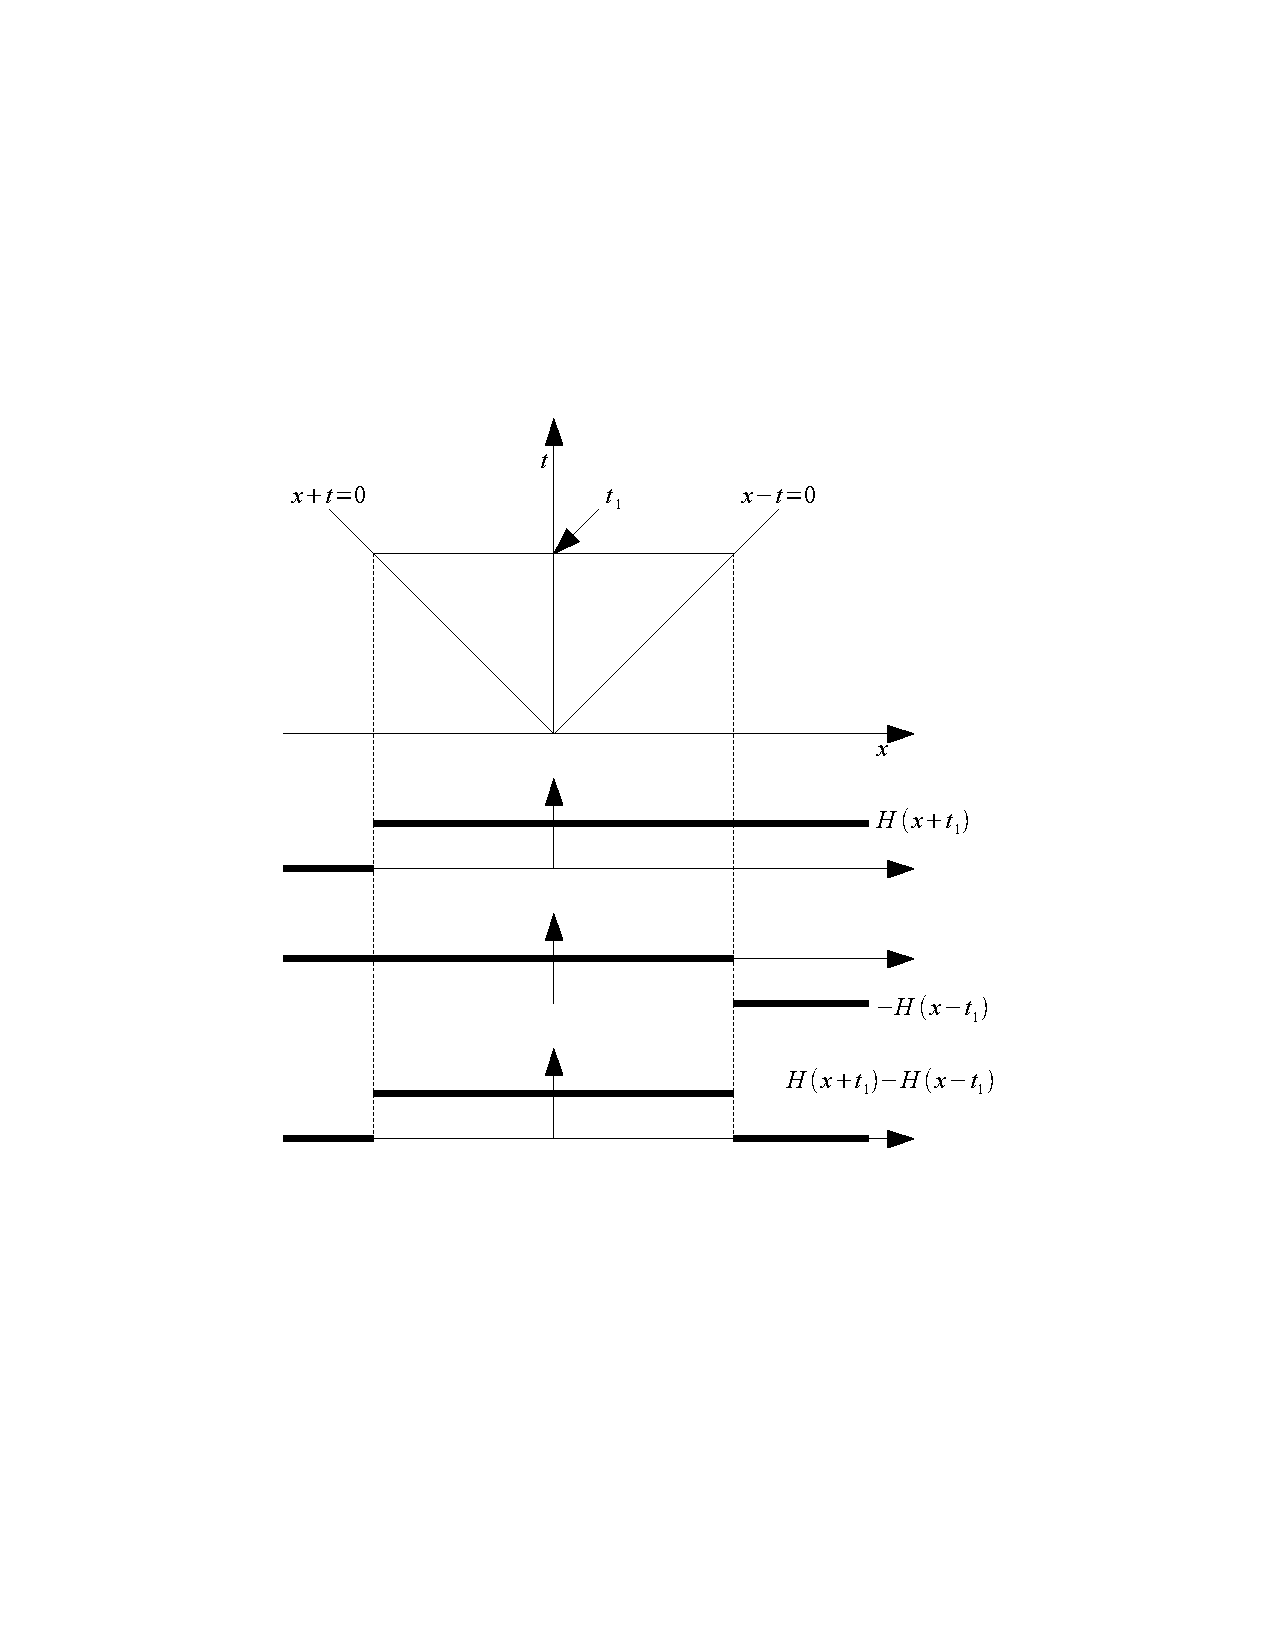
\includegraphics[height=0.95\textheight]{FIGS/xct}
\end{center}
}

\frame{
As $t$ increases, we move further up in the top graph in $(x,t)$-space, resulting in a wider and wider square pulse.
\begin{center}
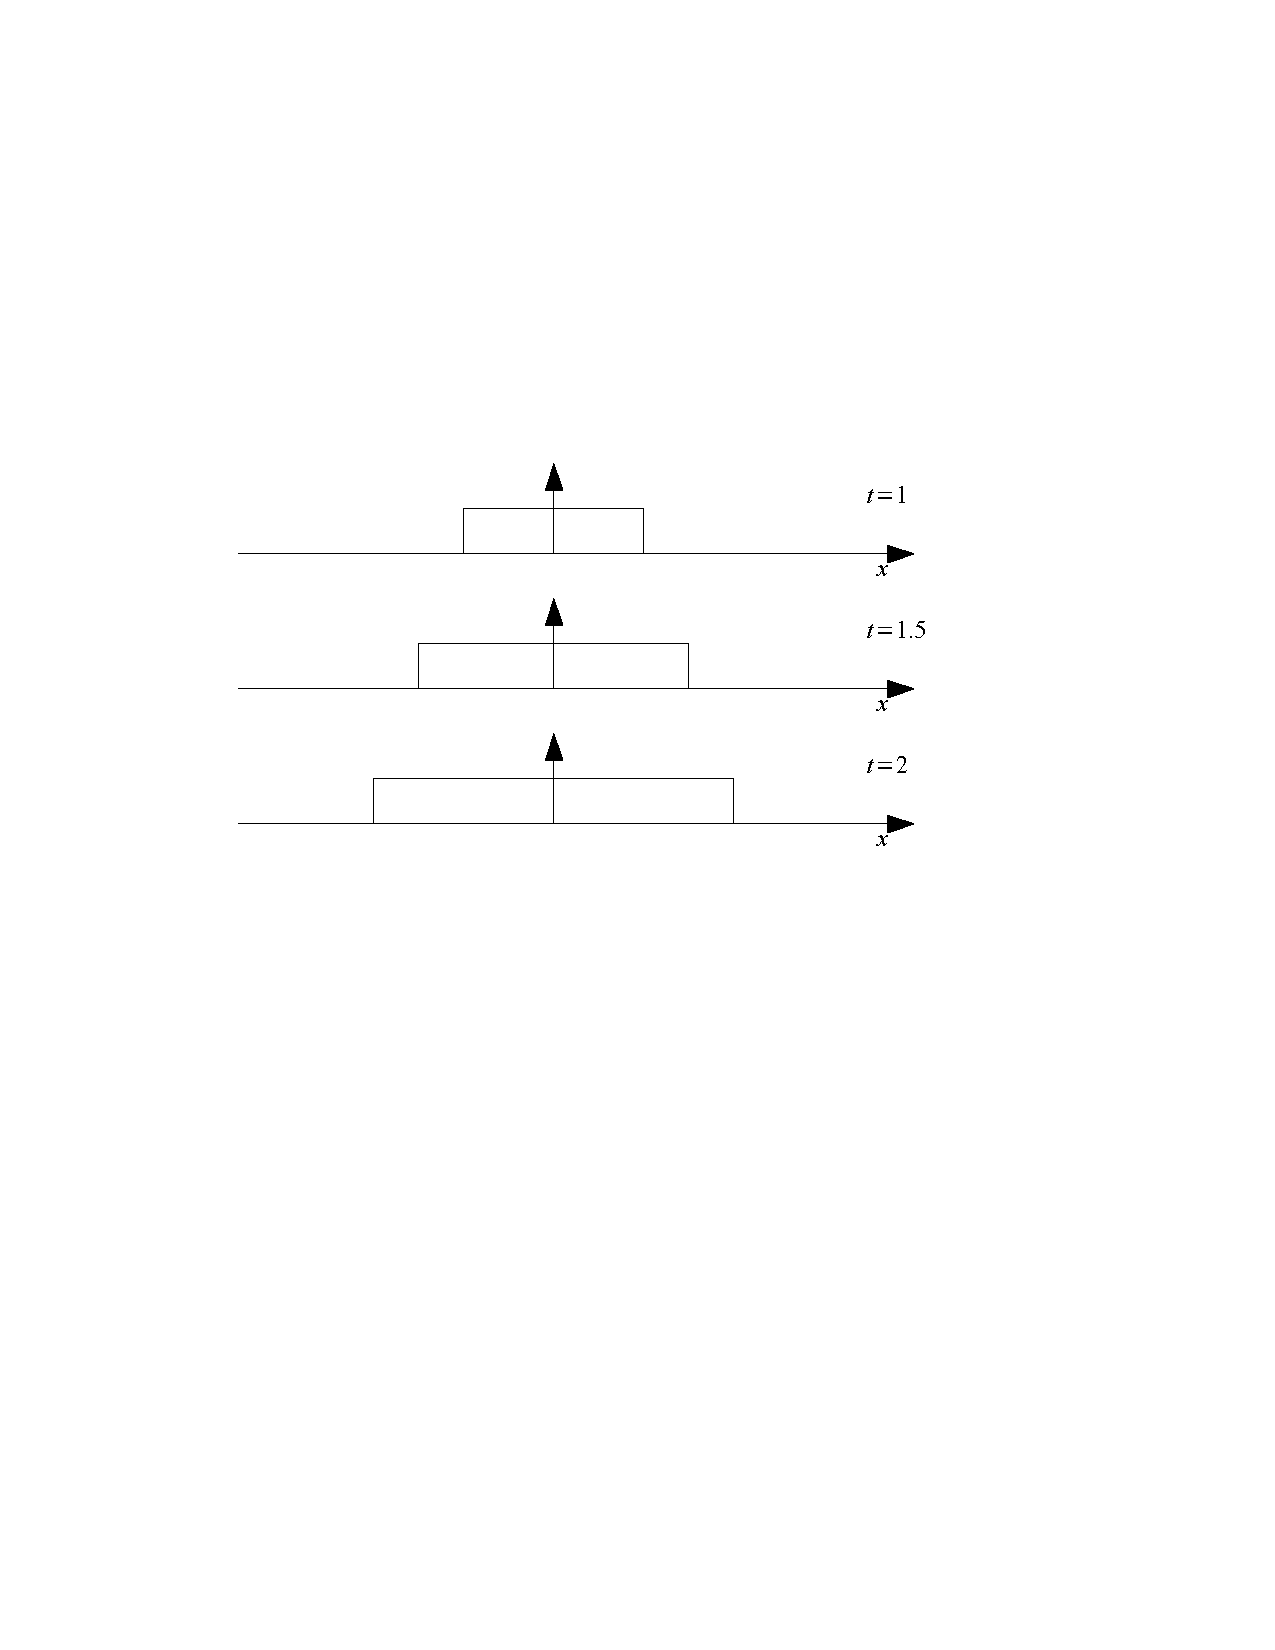
\includegraphics[width=\textwidth]{FIGS/xwave}
\end{center}
}

\end{document}
